\chapter{Algorytm odpornej optymalizacji regeneracyjnej}
\thispagestyle{chapterBeginStyle}
\label{ch:binaryIncMST}

W tym rozdziale skonstruujemy efektywny algorytm rozwiązujący jedno z zagadnień odpornej optymalizacji dyskretnej --- problem minimalnego drzewa rozpinającego dla okresowo zmieniających się kosztów z ograniczoną możliwością modyfikacji pierwotnego rozwiązania (problem \textsc{incremental minimum spanning tree}). Mając w ręku odpowiednie narzędzia przekonamy się, że konstrukcja takiego algorytmu jest prosta, w oparciu o wcześniej przedstawione pomysły będziemy mogli sprowadzić całe zagadnienie do prostego wyszukiwania binarnego, pokazać słuszność takiego postępowania oraz sposoby na jego udoskonalenie.

\section{Konstrukcja algorytmu i warunki optymalności}

Konstruowanie algorytmu rozwiązującego zagadnienie typu \textsc{incremental} dla minimalnego drzewa rozpinającego rozpoczniemy od powtórzenia (\ref{eq:imstcosts:e}) wyniku, otrzymanego w poprzednim rozdziale po zastosowaniu relaksacji Lagrange'a dla modelu \ref{mod:mst4}:

\begin{eqnarray}\label{eq:imstcosts2}
	\min \left\{ \sum_{e_{i} \in E \setminus T^{\ast}_{\textbf{s}}} c_{i} \cdot x_{i} + \sum_{\mathclap{e_{i} \in T^{\ast}_{\textbf{s}}}} \left( c_{i} - \lambda \right) \cdot x_{i} \right\}\text{,}
\end{eqnarray}
gdzie przypomnijmy, że $T^{\ast}_{\textbf{s}}$ oznaczał zbiór krawędzi należący do optymalnego rozwiązania problemu minimalnego drzewa rozpinającego dla starych kosztów w grafie, zdefiniowanych pzez scenariusz $\textbf{s}$.

Pokazaliśmy, że dla problemu minimalnego drzewa rozpinającego w wersji \textsc{inremental} z początkowym minimalnym drzewem rozpinającym $T^{\ast}_{\textbf{s}}$ i parametrem $k$ przedstawiającym liczbę dopuszczalnych zmian krawędzi względem pierwotnego rozwiązania, w wyniku zmiany kosztów w grafie, z twierdzenia o różnicach dopełniających zastosowanego do tak opisanego problemu (\ref{eq:imstcompl}), wynika że optymalnym jego rozwiązaniem jest zbiór krawędzi, który zawiera dokładnie $k$ łuków nie należących do początkowego rozwiązania $T^{\ast}_{\textbf{s}}$. Otrzymany wynik jest w pełni zgodny z tym, czego byśmy oczekiwali podchodząc do zadanego problemu, opierając się tylko o nasze intuicje --- niech $N \left( T, k \right)$ oznacza zbiór wszystkich drzew rozpinających różniących się od drzewa $T$ co najwyżej $k$ krawędziami, w szczególności $N \left( T, 0 \right) = \left\{ T \right\}$. Niech dane będzie $k^{\prime} < k$. Nietrudno zauważyć, że $N \left( T, k^{\prime} \right) \supseteq N \left( T, k \right)$, zatem jeżeli optymalne rozwiązanie problemu \textsc{imst} $T^{\ast}$ znajduje się w zbiorze $N \left( T, k^{\prime} \right)$, tym bardziej zawiera się w zbiorze większym --- $N \left( T, k \right)$. Odwrotna relacja oczywiście nie zachodzi --- rozwiązanie należące do zbioru $N \left( T, k \right)$, niekoniecznie musi należeć także do zbioru mniejszego. Aby zatem mieć pewność, że znajdziemy rozwiązanie optymalne dla problemu \textsc{imst} z parametrem $k$, musimy szukać go wśród drzew rozpinających graf o takiej samej liczbie nowych krawędzi względem starego rozwiązania (innymi słowy, co wydaje się oczywiste, wśród wszystkich możliwych dopuszczalnych rozwiązań problemu, a te należą do zbioru $N \left( T, k \right)$ --- rozwiązania, które charakteryzują się większą liczbą łuków niż $k$ są niedopuszczalne). Opierając się o wcześniej przypomniany wzór \ref{eq:imstcosts2} możemy zatem zauważyć, że rozsądną strategią na szukanie optymalnego rozwiązania dla badanego zagadnienia jest taka manipulacja parametrem $\lambda$, aby tak zdefiniowane tymczasowe koszty grafu dla nowego scenariusza $\textbf{s}^{\prime}$:

\begin{equation}
c^{\textbf{s}^{\prime} \left( \lambda \right)}_{i} = \left\{\begin{matrix}
c^{\textbf{s}^{\prime}}_{i} & \text{gdy $e_{i}$ nie należy do $T^{\ast}_{\textbf{s}}$,}\\ 
c^{\textbf{s}^{\prime}}_{i} - \lambda &  \text{gdy $e_{i}$ jest krawędzią należącą do oryginalnego rozwiązania,}
\end{matrix}\right.
\end{equation}
dla każdej krawędzi w grafie stopniowo wymuszały na algorytmie rozwiązującym problem minimalnego drzewa rozpinającego rozwiązania, których część wspólna ze starym rozwiązaniem jest coraz większa. Innymi słowy, zmniejszając koszty poszczególnych krawędzi w grafie podnosimy ich szansę na to, że znajdą się w zbiorze krawędzi minimalnego drzewa rozpinającego, jako że ich koszty w pewnym momencie staną się mniejsze od tych, które do tej pory trafiały do tego zbioru. Taką sytuację (oraz problemy związane z takim podejściem) doskonale odzwierciedlają rysunki od \ref{fig:imstExample:a} do \ref{fig:imstExample:f}. Przypomnijmy tylko, że liniami ciągłymi dla problemu \textsc{imst} oznaczaliśmy oryginalne minimalne drzewo rozpinające $T^{\ast}_{\textbf{s}}$, zaś kolorem czarnym --- aktualnie przedstawiane na rysunku rozwiązanie (to znaczy, że czarną linią przerywaną są zaznaczone te krawędzie, które w wyniku zmiany kosztów krawędzi w grafie weszły do rozwiązania problemu \textsc{imst} $T^{\ast}$ i nie należą do $T^{\ast}_{\textbf{s}}$, zaś szara linia ciągła oznacza krawędź, która z tych samych przyczyn nie należy do znalezionego rozwiązania, jest natomiast elementem zbioru $T^{\ast}_{\textbf{s}}$). Pozwoli nam to na łatwe stwierdzenie, czy przedstawiane rozwiązanie jest dopuszczalne, optymalne, czy nie należące do zbioru dopuszczalnych rozwiązań (odpowiednio $f \left( T^{\ast}, T^{\ast}_{\textbf{s}} \right) = \left| T^{\ast} \setminus T^{\ast}_{\textbf{s}} \right| = \left| T^{\ast}_{\textbf{s}} \setminus T^{\ast} \right| \leqslant k$, $f \left( T^{\ast}, T^{\ast}_{\textbf{s}} \right) = k$, $f \left( T^{\ast}, T^{\ast}_{\textbf{s}} \right) > k$).

\begin{figure}[!htbp]
	\null\hfill
	\begin{subfigure}[b]{0.32\textwidth}
		\includegraphics[width=\textwidth]{Chapter_IV/INC-MST-example/a}
		\caption{}
		\label{fig:imstExample:a}
	\end{subfigure}
	\hfill
	\begin{subfigure}[b]{0.32\textwidth}
		\includegraphics[width=\textwidth]{Chapter_IV/INC-MST-example/b}
		\caption{}
		\label{fig:imstExample:b}
	\end{subfigure}
	\hfill\null
	\caption{
		\textbf{(a)}~Optymalne rozwiązanie problemu \textsc{mst} dla scenariusza $\textbf{s} = \left[ 1, 2, 3, 7, 1, 3, 8, 4, 5 \right]$. Całkowity jego koszt wynosi $13$. Krawędzie do niego należące tworzą początkowe rozwiązanie dla problemu \textsc{imst} z parametrem $k = 1$: $T^{\ast}_{\textbf{s}} = \left\{ e_{1}, e_{2}, e_{5}, e_{8}, e_{9} \right\}$.
		\textbf{(b)}~Nieograniczone parametrem $k$, optymalne rozwiązanie problemu \textsc{mst} dla scenariusza $\textbf{s}^{\prime} = \left[ \textit{4}, 2, \textit{5}, 7, \textit{7}, 3, \textit{4}, 4, 5 \right]$, gdzie pochyloną czcionką zaznaczono wagi krawędzi, które uległy zmianie względem scenariusza $\textbf{s}$. Wartość takiego rozwiązania wynosi $17$ i jest tym samym rozwiązaniem jakie otrzymalibyśmy dla scenariusza $s^{\prime} \left( \lambda \right)$ w przypadku, gdy $\lambda = 0$. Należące do tego rozwiązania krawędzie tworzą zbiór $T^{\ast}_{\textbf{s}^{\prime}} = \left\{ e_{1}, e_{2}, e_{6}, e_{7}, e_{8} \right\}$, gdzie krawędzie $e_{6}$ i $e_{7}$ nie należą do $T^{\ast}_{\textbf{s}}$ ($f \left( T^{\ast}_{\textbf{s}^{\prime}}, T^{\ast}_{\textbf{s}} \right) = 2 > k$).
	}
\end{figure}

\begin{figure}[!htbp]
	\ContinuedFloat
	\null\hfill
	\begin{subfigure}[b]{0.32\textwidth}
		\includegraphics[width=\textwidth]{Chapter_IV/INC-MST-example/c1}
		\caption{}
		\label{fig:imstExample:c}
	\end{subfigure}
	\hfill
	\begin{subfigure}[b]{0.32\textwidth}
		\includegraphics[width=\textwidth]{Chapter_IV/INC-MST-example/c2}
		\caption{}
		\label{fig:imstExample:d}
	\end{subfigure}
	\hfill\null
	\caption{
		\textbf{(c)}~Rozwiązanie optymalne problemu \textsc{mst} dla wygenerowanego scenariusza $\textbf{s}^{\prime} \left( \lambda_{1} \right) = \left[ \textbf{3}, \textbf{1}, 5, 7, \textbf{6}, 3, 4, \textbf{3}, \textbf{4} \right]$, gdzie pogrubioną czcionką zaznaczono, obniżone o współczynnik $\lambda_{1}$ względem scenariusza $s^{\prime}$ i rozwiązania początkowego $T^{\ast}_{\textbf{s}}$, koszty na podstawie których algorytm rozwiązujący problem minimalnego drzewa rozpinającego zwrócił nam przedstawione rozwiązanie $T^{1} = \left\{ e_{1}, e_{2}, e_{6}, e_{7}, e_{8} \right\}$. Fikcyjny koszt takiego rozwiązania wynosi $14$.
		\textbf{(d)}~Inne optymalne rozwiązanie dla scenariusza $\textbf{s}^{\prime} \left( \lambda_{1} \right)$.
	}
\end{figure}

Po przyjrzeniu się bliżej rysunkom \ref{fig:imstExample:c} oraz \ref{fig:imstExample:d} zauważamy pierwszy poważny problem w naszej strategii --- algorytm do rozwiązywania problemu minimalnego drzewa rozpinającego (w tym przypadku celowo zastosowaliśmy algorytm Prima) ma skłonność do zwracania różnych odpowiedzi. Co gorsza, w kontekście problemu \textsc{imst} rozwiązania te nie są takie same, pomimo że ich koszt jest identyczny. Zauważmy, że o ile w przypadku \ref{fig:imstExample:c} dla scenariusza $\textbf{s}^{\prime} \left( 1 \right)$ zostało zwrócone identyczne rozwiązanie co na rysunku \ref{fig:imstExample:b} (niedopuszczalne, jako że zawierające więcej niż jedną krawędź nienależącą do $T^{\ast}_{\textbf{s}}$), to już rozwiązanie zwrócone na rysunku \ref{fig:imstExample:d} jest rozwiązaniem dopuszczalnym (co więcej, na mocy wcześniejszych lematów jest ono rozwiązaniem optymalnym). Skąd wzięła się ta różnica? Jeśli wrócimy do przedstawionego pseudokodu (\ref{alg:prime}), zobaczymy że algorytm Prima jako parametr wejściowy przyjmuje arbitralnie wybrany przez nas węzeł początkowy. Jako że w przypadku klasycznego problemu minimalnego drzewa rozpinającego jesteśmy zainteresowani jedynie sumą kosztów krawędzi zwracanego rozwiązania, nie ma dla nas różnicy, od którego węzła algorytm zacznie jego konstruowanie (zwykle po prostu jest to pierwszy węzeł, jeśli wierzchołki grafu przechowujemy w dowolny sposób uporządkowanej strukturze danych). Skutkuje to, tak jak pokazano na rysunkach \ref{fig:imstExample:c} i \ref{fig:imstExample:d}, w przypadku których wierzchołkami startowymi są odpowiednio wierzchołki $v_{1}$ i $v_{6}$, dwoma różnymi rozwiązaniami. Jakby tego było mało, na rysunkach \ref{fig:imstExample:e} i \ref{fig:imstExample:f} przedstawiono podobną sytuację, w której dla tego samego parametru $\lambda_{2} = 4$, znalezionymi rozwiązaniami są odpowiednio: rozwiązanie optymalne $T^{2} = \left\{ e_{1}, e_{2}, e_{5}, e_{8}, e_{9} \right\}$ o koszcie równym $18$ oraz dopuszczalne o sumie kosztów krawędzi należących do rozwiązania równej $22$ (koszt obydwu rozwiązań dla tymczasowego scenariusza $\textbf{s}^{\prime} \left( \lambda_{2} \right)$ są identyczne i wynoszą $2$). Ponownie otrzymaliśmy dwa różne rozwiązania tylko dlatego, że za początkowy wierzchołek obraliśmy $v_{1}$ (rysunek \ref{fig:imstExample:e}) oraz $v_{2}$ (\ref{fig:imstExample:f}).

\begin{figure}[!htbp]
	\ContinuedFloat
	\null\hfill
	\begin{subfigure}[b]{0.32\textwidth}
		\includegraphics[width=\textwidth]{Chapter_IV/INC-MST-example/d1}
		\caption{}
		\label{fig:imstExample:e}
	\end{subfigure}
	\hfill
	\begin{subfigure}[b]{0.32\textwidth}
		\includegraphics[width=\textwidth]{Chapter_IV/INC-MST-example/d2}
		\caption{}
		\label{fig:imstExample:f}
	\end{subfigure}
	\hfill\null
	\caption{
		\textbf{(e)}~Minimalne drzewo rozpinające grafu dla parametru $\lambda_{2} = 4$ i wygenerowanego na jego podstawie scenariusza $\textbf{s}^{\prime} \left( \lambda_{2} \right) = \left[ \textbf{0}, \textbf{-2}, 5, 7, \textbf{3}, 3, 4, \textbf{0}, \textbf{1} \right]$).
		\textbf{(f)}~Inne optymalne rozwiązanie dla scenariusza $\textbf{s}^{\prime} \left( \lambda_{2} \right)$. Koszt optymalnego rozwiązania wynosi $2$.
	}
	\label{fig:imstExample}
\end{figure}

Widzimy zatem, że tak opisana strategia szukania rozwiązania dla problemu \textsc{imst} posiada wadę, która czyni naszą strategię bezużyteczną, jako że typ zwracanego rozwiązania (optymalny, dopuszczalny bądź niedopuszczalny) nie zależy w pełni od świadomie wybieranego parametru $\lambda$ lecz od pośredniczącego algorytmu wyliczającego minimalne drzewo rozpinające. Należy podkreślić, że problem ten nie dotyczy tylko algorytmu Prima --- zdecydowaliśmy się na ten algorytm, gdyż na jego przykładzie najdokładniej widać istotę problemu. Problem ten będzie występował (może występować) zawsze, gdy w grafie, dla którego chcemy znaleźć minimalne drzewo rozpinające, będą występować co najmniej dwie krawędzie o takich samych kosztach, niezależnie od wybranego algorytmu.

\section{Struktura drzewa i koszty krawędzi}

Aby rozwiązać powyższy problem, będziemy chcieli zaburzyć koszty grafu w taki sposób, aby zapewnić sobie unikalność wag wszystkich krawędzi w grafie, nie zaburzając jednocześnie ich kolejności występowania tj. dla grafu $G = \left(V, E \right)$ i dla kosztów krawędzi w grafie $\textbf{s} = \left[ c_{i} : \forall e_{i} \in E \right]$, gdzie załóżmy dodatkowo, że $\exists e, e^{\prime} \in E \; : \; c_{e} = c_{e^{\prime}} \wedge e \neq e^{\prime}$, będziemy chcieli wygenerować nowe koszty $\textbf{s}^{\prime} = \left[ c^{\prime}_{i} : \forall e_{i} \in E \right]$, takie że $\forall e, e^{\prime} \in E \; : \; e \neq e^{\prime} \implies c^{\prime}_{e} \neq c^{\prime}_{e^{\prime}}$ a dodatkowo $\forall e, e^{\prime} \in E \; : \; c_{e} < c_{e^{\prime}} \implies c^{\prime}_{e} < c^{\prime}_{e^{\prime}}$. Zanim jednak zdefiniujemy takie przekształcenie, poczyńmy inną obserwację.

\begin{lemma}~\cite{incNetOpt}\label{lm:shrunkenGraph}
	Niech drzewa $T^{\ast}_{\textbf{s}}$ i $T^{\ast}_{\textbf{s}^{\prime}}$ oznaczają odpowiednio optymalne rozwiązania dla problemu \textsc{mst} i scenariuszy $\textbf{s}$ oraz $\textbf{s}^{\prime}$ problemu minimalnego drzewa rozpinającego w wersji \textsc{incremental} z parametrem $k$. Dla dowolnego $T^{\ast}_{\textbf{s}^{\prime}}$ w grafie $G = \left( V, E \right)$ istnieje minimalne drzewo rozpinające dla problemu \textsc{incremental} $T^{k}$ takie, że wszystkie jego krawędzie należą do zbioru $E^{\ast} = T^{\ast}_{\textbf{s}^{\prime}} \cup T^{\ast}_{\textbf{s}}$.
\end{lemma}

Z lematu zatem wynika, że aby znaleźć optymalne rozwiązanie dla problemu \textsc{imst}, możemy zamiast grafu $G = \left( V, E \right)$, wziąć pod uwagę dużo rzadszy graf $G^{\ast} = \left( V, E^{\ast} \right)$. Wynika to z faktu, że o ile istnieje optymalne rozwiązanie $T^{k}$ dla omawianego problemu w grafie $G$, takie samo rozwiązanie istnieje w $G^{\ast}$, zaś po drodze do rozwiązania ani razu nie będziemy brali pod uwagę krawędzi spoza zbioru $E^{\ast}$ (upraszczając, naszym celem jest wyjście od rozwiązania optymalnego $T^{\ast}_{\textbf{s}^{\prime}}$ dla nowego scenariusza $s^{\prime}$ i stopniowe zamienianie wybranych jego krawędzi na te należące do drzewa $T^{\ast}_{\textbf{s}}$ --- nie ma więc mowy, abyśmy potrzebowali krawędzi spoza zbioru $T^{\ast}_{\textbf{s}^{\prime}} \cup T^{\ast}_{\textbf{s}} = E^{\ast}$). Ta obserwacja pozwala nam często w znacznym stopniu zredukować strukturę grafu, gdyż w najgorszym przypadku moc nowo otrzymanego zbioru krawędzi będzie wynosić $\left| E^{\ast} \right| = 2 \cdot n - 2$ (w przypadku gdy oba zbiory krawędzi są rozłączne, zaś każdy z nich z definicji bycia drzewem zawiera dokładnie $\left| V \right| - 1$ krawędzi, gdzie $\left| V \right| = n$). Nawet w takim przypadku, nasza obserwacja może okazać się wielce pomocna, na przykład gdy mamy do czynienia z grafem pełnym --- w takim przypadku możemy mówić o zredukowaniu mocy zbioru krawędzi do co najmniej $\frac{2 \cdot \left( n - 1 \right)}{\binom{n}{2}} = \frac{4}{n}$ części jego oryginalnej liczebności.

\begin{proof}
	Niech drzewa $T^{\ast}_{\textbf{s}}$ i $T^{\ast}_{\textbf{s}^{\prime}}$ będą zdefiniowane tak jak w lemacie. Dodatkowo niech $T^{k}$ będzie optymalnym rozwiązaniem dla problemu minimalnego drzewa rozpinającego w wersji \textsc{incremental}, takim że zawiera ono największą liczbę krawędzi ze zbioru $E^{\ast}$ spośród pozostałych rozwiązań. Jeśli liczba takich krawędzi w drzewie $T^{k}$ równa się jego mocy ($\left| T^{k} \right| = n - 1$) to dowód możemy zakończyć, gdyż $\forall e \in T^{k} \; \left( e \in T^{k} \implies e \in E^{\ast} \right)$, więc $T^{k} \subseteq E^{\ast}$.
	
	Załóżmy zatem, że tak nie jest, czyli że istnieje taka krawędź $e \in T^{k}$, która nie należy do zbioru $E^{\ast}$ --- $e \in T^{k} \setminus E^{\ast}$. Aby $T^{k} \subseteq E^{\ast}$, usuńmy z niego tą krawędź. W wyniku usunięcia krawędzi $e$ z drzewa $T^{k}$ otrzymamy podział na dwa zbiory krawędzi będące drzewami: $S$ i $\overline{S}$ oraz zbiór $\mathcal{Q} \left( T^{k}, e \right)$ (zbiór zdefiniowaliśmy w \ref{eq:treecutedgeset} i oznaczał on zbiór wszystkich takich krawędzi $e_{ij}$, gdzie $v_{i} \in S$ oraz $v_{j} \in \overline{S}$). Skorzystajmy teraz z własności optymalnego cięcia (\ref{def:optmstcut}), które mówi, że drzewo jest minimalnym drzewem rozpinającym $T$ wtedy i tylko wtedy, gdy należące do niego krawędzie $e^{\prime}$ mają najmniejszy koszt spośród wszystkich innych krawędzi, które należą do zbiorów $\mathcal{Q} \left( T, e^{\prime} \right)$ (dla każdej krawędzi $e^{\prime} \in T$). Wybierzmy zatem ze zbioru $\mathcal{Q} \left( T^{k}, e \right)$ krawędź $e^{\ast}$ o najmniejszym koszcie w tym zbiorze. Bezpośrednio z powyższej własności wiemy, że wybrana krawędź należy do minimalnego drzewa rozpinającego $T^{\ast}_{\textbf{s}^{\prime}}$. W związku z tym, że usuwana z drzewa $T^{k}$ krawędź $e \notin E^{\ast}$, z definicji $e \notin T^{\ast}_{\textbf{s}^{\prime}} \wedge e \notin T^{\ast}_{\textbf{s}}$. Z faktu zaś, że $e \notin T^{\ast}_{\textbf{s}^{\prime}}$ otrzymujemy natychmiast prosty wniosek, że $e \neq e^{\ast}$ ($e \notin T^{\ast}_{\textbf{s}^{\prime}}$, $e^{\ast} \in T^{\ast}_{\textbf{s}^{\prime}}$). W związku z tym nic nie stoi na przeszkodzie aby z drzewa $T^{k}$ stworzyć nowe drzewo $T^{k\prime}$, różne od $T^{k}$, poprzez usunięcie krawędzi $e \in T^{k} \setminus E^{\ast}$ a dodanie do niego $e^{\ast} \in T^{\ast}_{\textbf{s}^{\prime}} \in E^{\ast}$. Zauważmy, że z własności $e^{\ast}$ wynika, że suma kosztów krawędzi w drzewie $T^{k\prime}$ jest co najwyżej równo tej samej wartości dla drzewa $T^{k}$. Jako że drzewo $T^{k}$ było rozwiązaniem optymalnym, nie istnieje drzewo o mniejszej sumie kosztów krawędzi do niego należących. Stąd prosty wniosek, że suma wag łuków w drzewie $T^{k\prime}$ jest taka sama jak w $T^{k}$. Dodatkowo oczywistym jest, że otrzymane drzewo nadal jest rozwiązaniem dopuszczalnym dla problemu \textsc{imst}. Z założenia optymalności $T^{k}$ i definicji problemu \textsc{incremental} mamy, że $f \left( T^{k}, T^{\ast}_{\textbf{s}} \right) = k$. Usuwana z drzewa $T^{k}$ krawędź $e \in T^{k} \setminus E^{\ast}$ z założenia nie należy do zbioru $T^{\ast}_{\textbf{s}}$, więc $f \left( T^{k} \setminus \left\{ e \right\}, T^{\ast}_{\textbf{s}} \right) = k - 1 < k$ (zatem bez względu na dodawaną krawędź $e^{\ast}$, drzewo $T^{k\prime}$ jest rozwiązaniem dopuszczalnym). Zatem, skoro nowe drzewo jest również rozwiązaniem dopuszczalnym i zarazem optymalnym, a przy okazji zawiera o jedną krawędź wspólną ze zbiorem $E^{\ast}$ niż drzewo $T^{k}$, otrzymaliśmy sprzeczność z założeniem, że $T^{k}$ zawiera największą liczbę takich krawędzi spośród wszystkich optymalnych rozwiązań, co kończy dowód.
\end{proof}

Tym samym od razu możemy zredukować wyprowadzone przez nas równanie \ref{eq:imstcosts2}, zauważając, że zbiór $E \setminus T^{\ast}_{\textbf{s}} = \left( T^{\ast}_{\textbf{s}} \cup T^{\ast}_{\textbf{s}^{\prime}} \right) \setminus T^{\ast}_{\textbf{s}} = T^{\ast}_{\textbf{s}^{\prime}$:

\begin{equation}\label{eq:imstcosts3}
	\min \left\{ \sum_{e_{i} \in E \setminus T^{\ast}_{\textbf{s}}} c_{i} \cdot x_{i} + \sum_{\mathclap{e_{i} \in T^{\ast}_{\textbf{s}}}} \left( c_{i} - \lambda \right) \cdot x_{i} \right\} = \min \left\{ \sum_{e_{i} \in T^{\ast}_{\textbf{s}^{\prime}}} c_{i} \cdot x_{i} + \sum_{\mathclap{e_{i} \in T^{\ast}_{\textbf{s}}}} \left( c_{i} - \lambda \right) \cdot x_{i} \right\}\text{.}
\end{equation}
	
Pokażemy teraz jak dla tak zredukowanego zbioru krawędzi (z $E$ do $E^{\ast}$) stworzyć sztuczny scenariusz, w którym wszystkie koszty krawędzi będą unikalne i jednocześnie zachowywały oryginalną relację w stosunku do pozostałych kosztów.

\begin{lemma}~\cite{Dimitromanolakis02analysisof}
	Dla danych kosztów krawędzi $c_{e_{i}}$ w grafie $G = \left( V, E \right)$, dla każdego $i \in \left\{ 1, \dots, \left| E \right| \right\}$ dla zmodyfikowanych kosztów zdefiniowanych jako $c^{\prime}_{e_{i}} = c_{e_{i}} + \phi \left( i \right)$, gdzie $\phi \left( i \right) = \frac{m \cdot i^{2} + i}{\left( m + 1 \right)^{3}}$, zachodzi:
	\begin{equation}\label{eq:Dimitromanolakis1}
		c_{e_{i}} < c^{\prime}_{e_{i}} < c_{e_{i}} + 1\text{,}
	\end{equation}
	gdzie $m = \left| E \right|$.
\end{lemma}

Dla tak zdefiniowanych kosztów dodatkowo pokażemy, że dla dowolnych $i$ oraz $j$, takich że $i \neq j$ zachodzi dodatkowa własność:

\begin{equation}\label{eq:Dimitromanolakis2}
	\forall e_{i}, e_{j} \in E \; \left( i \neq j \implies c^{\prime}_{e_{i}} \neq c^{\prime}_{e_{j}} \right)\text{.}
\end{equation}

Dzięki tym dwóm własnościom będziemy mieli pewność, że po nałożeniu na wszystkie krawędzie w grafie takiego wzoru, każda krawędź będzie miała unikalny koszt, zaś po uporządkowaniu krawędzi względem ich kosztów oryginalnych i zaburzonych, otrzymamy wa identyczne ciągi (w wyniku zaburzenia kosztów, koszt żadnej z krawędzi nie przewyższy ani nie zostanie przewyższony przez koszt innej, której oryginalna waga przewyższała lub była przewyższana przez koszt pierwszej z nich). Taka modyfikacja rozwiąże obydwa problemy, o których wspomnieliśmy przy omawianiu rysunków od \ref{fig:imstExample:c} do \ref{fig:imstExample:f}. Oczywiście takie podejście niesie za sobą pewne ograniczenia --- oryginalne koszty krawędzi muszą być całkowitoliczbowe, gdyż w przeciwnym przypadku własność \ref{eq:Dimitromanolakis1} nie będzie dawała nam żadnej gwarancji, że dla zmodyfikowanych kosztów będziemy otrzymywać te same rozwiązania problemu drzewa rozpinającego co dla kosztów oryginalnych. Jeżeli zależy nam na zachowaniu zmiennoprzecinkowych wag na krawędziach --- możemy albo dodatkowo zmodyfikować koszty początkowe poprzez pomnożenie ich przed odpowiednią potęgę liczby $10$, bądź też wprowadzić odgórny porządek na krawędziach, co wiązać się dodatkowo będzie z koniecznością modyfikacji każdej części naszych algorytmów, w których stają one przed wyborem jednej z dwóch lub większej liczby krawędzi o tym samym koszcie.

\begin{proof}
	Dowód własności \ref{eq:Dimitromanolakis1} sprowadzimy do problemu pokazania, że dla dowolnego parametru, wartość $\phi \left( i \right)$ zawiera się w przedziale otwartym $\left( 0, 1 \right)$. Niech zatem $\phi \left( i \right) = \frac{m \cdot i^{2} + i}{\left( m + 1 \right)^{3}}$, gdzie $m = \left| E \right|$.
	\begin{gather}
		c_{e_{i}} < c^{\prime}_{e_{i}} < c_{e_{i}} + 1\text{,}\nonumber\\
		0 < \left( c_{e_{i}} + \phi \left( i \right) \right) - c_{e_{i}} < 1\text{,}\nonumber\\
		0 < \frac{m \cdot i^{2} + i}{\left( m + 1 \right)^{3}} < 1\text{,}\label{eq:DimitromanolakisProof1}\\
		0 < m \cdot i^{2} + i < \left( m + 1 \right)^{3}\text{,}\nonumber\\
		0 < m \cdot i^{2} + i \leqslant m^{3} + m < m^{3} + 3 \cdot m^2 + 3 \cdot m + 1 = \left( m + 1 \right)^{3}\nonumber\text{.}
	\end{gather}
	W ostatniej nierówności skorzystaliśmy z faktu, że $i$ oznacza numer porządkowy krawędzi w grafie, $i \in \left\{ 1, \dots, m \right\}$. Pokażemy teraz dodatkową własność \ref{eq:Dimitromanolakis2} dla dowolnego $i \neq j$:
	\begin{gather}
		c^{\prime}_{e_{i}} \neq c^{\prime}_{e_{j}}\text{,}\nonumber\\
		c_{e_{i}} + \phi \left( i \right) \neq c_{e_{j}} + \phi \left( j \right)\text{,}\nonumber\\
		c_{e_{i}} + \frac{m \cdot i^{2} + i}{\left( m + 1 \right)^{3}} \neq c_{e_{j}} + \frac{m \cdot j^{2} + j}{\left( m + 1 \right)^{3}}\text{.}\label{eq:DimitromanolakisProof2}
	\end{gather}
	Jeżeli $c_{e_{i}} = c_{e_{j}}$, \ref{eq:DimitromanolakisProof2} w oczywisty sposób jest spełnione. W przeciwnym przypadku mamy spełniony warunek $c_{e_{i}} + 1 \leqslant c_{e_{j}}$ (zakładając bez straty ogólności, że uporządkowaliśmy koszty rosnąco według numeru porządkowego krawędzi a $i < j$ oraz, że kosztami są liczby całkowite) i stosując \ref{eq:DimitromanolakisProof1} otrzymamy:
	\begin{gather*}
		c_{e_{i}} < c_{e_{i}} + \frac{m \cdot i^{2} + i}{\left( m + 1 \right)^{3}} < c_{e_{i}} + 1 \leqslant c_{e_{j}} < c_{e_{j}} + \frac{m \cdot j^{2} + j}{\left( m + 1 \right)^{3}}\text{.}
	\end{gather*}
\end{proof}

Pokazaliśmy zatem poprawność jednego ze sposobów na rozwiązanie problemu z nieunikatowymi kosztami krawędzi w grafie, a co za tym idzie --- zapewnić jednoznaczność rozwiązań zwracanych przez algorytm Prima (bądź inny rozwiązujący zagadnienie minimalnego drzewa rozpinającego) dla dowolnego scenariusza i dowolnej wartości parametru $\lambda$. Przyglądając się formule \ref{eq:imstcosts2}, doszliśmy też do wniosku, że wraz ze stopniowym zwiększaniem wartości tego parametru otrzymujemy kolejne rozwiązania, którym coraz bliżej do spełnienia warunków, które określiliśmy w poprzednim rozdziale (\ref{eq:imstoptcond1}, \ref{eq:imstoptcond2}). Pokażemy teraz formalnie, że takie postępowanie istotnie doprowadzi nas do rozwiązania.

\begin{theorem}~\cite[$589$]{incNetOpt}\label{th:incNetOpt}
	Drzewo rozpinające $T^{\ast}$ jest unikalnym minimalnym drzewem rozpinającym dla problemu \textsc{incremental} wtedy i tylko wtedy, gdy spełnia własności \ref{eq:Dimitromanolakis1}, \ref{eq:Dimitromanolakis2} oraz istnieje parametr $\lambda \geqslant 0$, dla którego $T^{\ast}$ jest optymalne oraz:
	\begin{align}
		f \left( T^{\ast}, T^{\ast}_{\textbf{s}} \right) \leqslant k \; & \wedge \; \lambda = 0 \quad \text{lub}\label{eq:imstoptcond3}\\
		f \left( T^{\ast}, T^{\ast}_{\textbf{s}} \right) = k \; & \wedge \; \lambda \neq 0\text{.}\label{eq:imstoptcond4}
	\end{align}
\end{theorem}

\begin{proof}
	Unikalność rozwiązania $T^{\ast}$ bezpośrednio wynika z własności \ref{eq:Dimitromanolakis2}, zaś pierwsza część dowodu (jeśli istnieje $\lambda \geqslant 0$, dla której $T^{\ast}$ jest optymalne i spełnione są warunki \ref{eq:imstoptcond3} i \ref{eq:imstoptcond4}, wtedy $T^{\ast}$ jest unikalnym minimalnym drzewem rozpinającym dla problemu \textsc{imst}) jest w zasadzie powtórzeniem twierdzenia o różnicach dopełniających , którego słuszność pokazaliśmy w poprzednim rozdziale (\ref{eq:imstcompl}). Pozostaje nam zatem do udowodnienia druga część dowodu (tylko wtedy, gdy istnieje $\lambda \geqslant 0$, dla której $T^{\ast}$ jest optymalne i spełnione są warunki \ref{eq:imstoptcond3} i \ref{eq:imstoptcond4}, $T^{\ast}$ jest unikalnym minimalnym drzewem rozpinającym dla problemu \textsc{imst}). Oczywiście, gdy $\lambda = 0$, drzewo $T^{\ast} = T^{\ast}_{\textbf{s}^{\prime}}$ jest minimalnym drzewem rozpinającym. Co więcej, jeżeli spełnia nierówność $f \left( T^{\ast}, T^{\ast}_{\textbf{s}} \right) \leqslant k$, jest także optymalnym rozwiązaniem dla problemu \textsc{imst}. Załóżmy zatem, że tak nie jest i $\left( T^{\ast}, T^{\ast}_{\textbf{s}} \right) = k^{\prime} > k$. Co powinno być już dla nas oczywiste, jeżeli zaczniemy zwiększać wartość parametru $\lambda$, równolegle do niej będziemy zmniejszać koszty wszystkich krawędzi $e \in T^{\ast}_{\textbf{s}}$. W pewnym momencie parametr $\lambda$ osiągnie taką wartość, że koszt pewnej pojedynczej krawędzi $e_{0} \in T^{\ast}_{\textbf{s}}$ zrówna się z kosztem krawędzi $e_{0}^{\ast}$ należącej do aktualnego rozwiązania. Niech wartość tą reprezentuje wyrażenie $\lambda_{1}$, zaś drzewo o kosztach krawędzi zależnych od niego --- $T \left( \lambda_{1} \right)$. Skoro $c_{e_{0}} - \lambda_{1} = c_{e_{0}^{\ast}}$, to zamieniając ze sobą krawędzie miejscami ($e_{0} \in T^{\ast}_{\textbf{s}} \setminus T \left( \lambda_{1} \right)$ dołączając do rozwiązania, zaś $e_{0}^{\ast} \in T \left( \lambda_{1} \right) \setminus T^{\ast}_{\textbf{s}}$ z niego usuwając), otrzymamy nowy zbiór krawędzi $E^{\prime} \left( \lambda_{1} \right)$\footnote{Trzeba tutaj zaznaczyć, że operacja wymiany krawędzi między zbiorami nic nie wspomina o własnościach dodawanego łuku względem starego --- nie jesteśmy zatem w stanie powiedzieć czy dodawana krawędź zapewni nam to, że nowy zbiór będzie nadal drzewem (np. należy do zbioru $\mathcal{Q} \left( T^{\ast} \left( \lambda_{1} \right), e_{0} \right)$, gdzie $e_{0}$ to krawędź usuwana, gdzie w takim przypadku na pewno otrzymalibyśmy nowe drzewo). Aby zapewnić sobie, że nowy zbiór będzie nadal drzewem, powinniśmy wartość parametru $\lambda_{1}$ (i każdy następny) podnieść jeszcze wyżej o $\epsilon$, a następnie poprosić algorytm dla problemu \textsc{mst} o nowe rozwiązanie.}, który będzie spełniał równość $f \left( E^{\prime} \left( \lambda_{1} \right), T^{\ast}_{\textbf{s}} \right) = k^{\prime} - 1$, zaś suma wszystkich krawędzi w nowym zbiorze będzie równa tej sumie w $T \left( \lambda_{1} \right)$ (z punktu widzenia algorytmu rozwiązującego problem \textsc{mst} nic więc się nie zmieni). Dodatkowo warto zauważyć, że ze względu na własności \ref{eq:Dimitromanolakis1} i \ref{eq:Dimitromanolakis2}, które założyliśmy że spełniają wszystkie krawędzie w grafie\footnote{Graf może zawierać już tylko łuki $E = T^{\ast}_{\textbf{s}^{\prime}} \cup T^{\ast}_{\textbf{s}}$.}, taka para krawędzi $\left( e_{0}, e_{0}^{\ast} \right)$ jest unikalna, więc w każdym kroku będziemy wymieniać co dokładnie jedną krawędź pomiędzy zbiorami. Powtarzając więc powyżej opisane kroki, podnosząc sukcesywnie wartość parametru $\lambda$, otrzymamy zbiór wartości $\lambda_{1}$, $\lambda_{2}$, $\dots$, $\lambda_{k^{\prime} - k}$ oraz analogicznie ciąg zbiorów $E^{\prime} \left( \lambda_{1} \right)$, $E^{\prime} \left( \lambda_{2} \right)$, $\dots$, $E^{\prime} \left( \lambda_{k^{\prime} - k} \right)$, gdzie każdy z nich spełnia równość $f \left( E^{\prime} \left( \lambda_{i} \right), T^{\ast}_{\textbf{s}} \right) = k^{\prime} - i$. To oznacza, że w którymś momencie (dokładnie dla $\lambda_{k^{\prime} - k}$) otrzymamy $f \left( E^{\prime} \left( \lambda_{k^{\prime} - k} \right), T^{\ast}_{\textbf{s}} \right) = k^{\prime} - \left( k^{\prime} - k \right) = k$ (widzimy, że funkcja $f : X \times X \rightarrow \NN$ jest monotoniczna, malejąca), co oznaczać będzie, że spełniliśmy jeden z dwóch opcjonalnych warunków optymalności rozwiązania (\ref{eq:imstoptcond4}).
\end{proof}

Mamy zatem pewność, że nasza strategia stopniowego zwiększania wartości parametru $\lambda$ i równoległego obniżania kosztów krawędzi, należących do oryginalnego rozwiązania $T^{\ast}_{\textbf{s}}$, doprowadzi nas do znalezienia optymalnego rozwiązania problemu minimalnego drzewa rozpinającego w wersji \textsc{incremental} z parametrem $k$. Pozostaje nam zatem już tylko kwestia odpowiedniego dobierania wartości wspomnianego parametru, jako że do tej pory milcząco zakładaliśmy, że zawsze jesteśmy w stanie znaleźć odpowiednie jego wartości (dla których każde kolejne rozwiązanie będzie zawierało malejącą liczbę krawędzi $e \notin T^{\ast}_{\textbf{s}}$, aż do momentu, gdy ich liczba wyniesie dokładnie $k$). Pierwszym naiwnym pomysłem jest oczywiście zadanie pewnego interwału $\Delta > 0$ i rozpoczęcie generowania kolejnych wartości parametru $\lambda$, rozpoczynając od $\lambda_{\text{min}}$, kończąc na pewnym $\lambda_{\text{max}}$ (gdzie $\lambda_{\text{min}}$ może równać się $0$ --- wtedy pierwsze wygenerowane drzewo $T \left( \lambda_{\text{min}} \right)$ odpowiadać będzie oczywiście drzewu $T^{\ast}_{\textbf{s}^{\prime}}$ ---  za $\lambda_{\text{max}}$ możemy przyjąć chociażby koszt krawędzi w grafie o największej wadze)\footnote{Jeśli dla zadanych danych problem minimalnego drzewa rozpinającego w wersji \textsc{incremental} ma rozwiązanie, najprawdopodobniej przerwiemy obliczenia poniżej wartości $\lambda_{\text{max}}$, jednakże w przeciwnym przypadku musimy takie górne ograniczenie przyjąć.}. Wtedy będziemy generować kolejne drzewa: $T \left( \lambda_{\text{min}} \right)$, $T \left( \lambda_{\text{min}} + \Delta \right)$, $\dots$, $T \left( \lambda_{\text{min}} + i \cdot \Delta \right) = T^{k}$, gdzie po $i$ iteracjach możemy natknąć się na pierwsze optymalne rozwiązanie $T^{k}$ dla badanego problemu. Problemy, które natychmiastowo pojawiają się przy takim rozwiązaniu są dwa. Nie potrafimy określić jakiego rzędu wielkości powinien być parametr $\Delta$, by przypadkiem nie ,,przeskoczyć'' odpowiednich wartości $\lambda$. Z drugiej strony, zmniejszanie tego pierwszego bardzo szybko zwiększa nam liczbę potencjalnych minimalnych drzew rozpinających, które musielibyśmy policzyć, co z kolei przekłada się negatywnie na czas działania takiego algorytmu.

\section{Binarne poszukiwanie rozwiązania}

Pierwszą próbą udoskonalenia przedstawionego pomysłu jest skorzystanie z własności funkcji $f$, która zwraca liczbę krawędzi będących częścią jednego z drzew, będącego parametrem tej funkcji, zaś nie należących do drzewa przekazanego jako jej drugi parametr. W dowodzie twierdzenia \ref{th:incNetOpt} pokazaliśmy, że wspomniana funkcja jest funkcją monotoniczną --- dla dwóch różnych parametrów $\lambda_{i}$, $\lambda_{j}$, gdzie $i < j$ ($\lambda_{i} < \lambda_{j}$) zachodzi $f \left( T \left( \lambda_{i} \right), T^{\ast}_{\textbf{s}} \right) \geqslant f \left( T \left( \lambda_{j} \right), T^{\ast}_{\textbf{s}} \right)$. W naszym przypadku $f \left( T \left( \lambda_{i} \right), T^{\ast}_{\textbf{s}} \right) \geqslant f \left( T \left( \lambda_{i} + \Delta \right), T^{\ast}_{\textbf{s}} \right)$, zaś w przypadku przytoczonych dowodów zakładaliśmy, że każdy kolejny parametr $\lambda$ spełniał $f \left( T \left( \lambda_{i} \right), T^{\ast}_{\textbf{s}} \right) < f \left( T \left( \lambda_{j} \right), T^{\ast}_{\textbf{s}} \right)$. Fakt takiego zachowania się funkcji $f$ prowadzi nas do pomysłu zastosowania dla badanego problemu wyszukiwania binarnego --- mając ciąg parametrów $\lambda_{0} < \lambda_{1} < \dots < \lambda_{i-1} < \lambda_{i} < \lambda_{i+1} < \dots \lambda_{\text{max}}$ (i odpowiadający im ciąg wartości funkcji $f \left( T \left( \lambda_{0} \right), T^{\ast}_{\textbf{s}} \right) \geqslant f \left( T \left( \lambda_{1} \right), T^{\ast}_{\textbf{s}} \right) \geqslant \dots \geqslant f \left( T \left( \lambda_{i-1} \right), T^{\ast}_{\textbf{s}} \right) \geqslant f \left( T \left( \lambda_{i} \right), T^{\ast}_{\textbf{s}} \right) \geqslant f \left( T \left( \lambda_{i+1} \right), T^{\ast}_{\textbf{s}} \right) \geqslant \dots \geqslant f \left( T \left( \lambda_{\text{max}} \right), T^{\ast}_{\textbf{s}} \right)$) łatwo zauważyć, że:

\begin{itemize}
	\item Jeśli $f \left( T \left( \lambda_{i} \right), T^{\ast}_{\textbf{s}} \right) > k$, wtedy dla każdego drzewa $T \left( \lambda_{j} \right)$, gdzie $j < i$ ($\lambda_{j} < \lambda_{i}$) zachodzić będzie $f \left( T \left( \lambda_{j} \right), T^{\ast}_{\textbf{s}} \right) > k$. Zatem z góry możemy powiedzieć, że minimalne drzewa rozpinające liczone dla wszystkich scenariuszy $\mathcal{S} = \left\{ \textbf{s}^{\prime} \left( \lambda_{j} \right) : j \leqslant i \right\}$ okażą się rozwiązaniami, które nie są nawet dopuszczalne.
	\item Jeśli $f \left( T \left( \lambda_{i} \right), T^{\ast}_{\textbf{s}} \right) < k$, wtedy dla każdego drzewa $T \left( \lambda_{j} \right)$, gdzie $j > i$ ($\lambda_{j} > \lambda_{i}$) zachodzić będzie $f \left( T \left( \lambda_{j} \right), T^{\ast}_{\textbf{s}} \right) < k$. Zatem ponownie możemy powiedzieć, że minimalne drzewa rozpinające liczone dla wszystkich scenariuszy $\mathcal{S} = \left\{ \textbf{s}^{\prime} \left( \lambda_{j} \right) : j \geqslant i \right\}$ będą rozwiązaniami dopuszczalnymi, lecz nie optymalnymi (ze względu na niespełnienie warunków twierdzenia \ref{th:incNetOpt}).
	\item Jeśli $f \left( T \left( \lambda_{i} \right), T^{\ast}_{\textbf{s}} \right) = k$, to znaleźliśmy rozwiązanie optymalne.
\end{itemize}

Dzięki takiemu podejściu, natychmiastowo redukujemy liczbę wymaganych obliczeń do logarytmu z tej liczby (tak jak to pokazano w pseudokodzie \ref{alg:binnarysearch}). Nadal jednak nie mamy żadnej gwarancji, że dobrana wartość parametru pomocniczego $\Delta$ zapewni nam prawidłowe działanie naszego algorytmu --- może się okazać, że podążając ścieżką wytyczoną przez algorytm \ref{alg:binnarysearch} dojdziemy do takiego momentu, w którym w rozpatrywanym przedziale $\left[ \lambda_{l}, \lambda_{l} + \Delta, \dots, \lambda_{h} - \Delta, \lambda_{h} \right]$ nie ma takiej wartości parametru $\lambda^{\ast}_{i}$, dla której otrzymalibyśmy rozwiązanie optymalne (takiego, że $f \left( T \left( \lambda^{\ast}_{i} \right), T^{\ast}_{\textbf{s}} \right) = k$), chociaż zgodnie z algorytmem są spełnione warunki: $f \left( T \left( \lambda_{l} \right), T^{\ast}_{\textbf{s}} \right) \geqslant k$ oraz $f \left( T \left( \lambda_{h} \right), T^{\ast}_{\textbf{s}} \right) \leqslant k$. Częściowym rozwiązaniem tego problemu jest pozwolenie algorytmowi w takiej sytuacji na porzucenie dyskretnego zbioru parametrów i samodzielne rozpoczęcie generowania nowych, będących średnimi arytmetycznymi wartości skrajnych kolejnych przedziałów. Takie rozwiązanie gwarantuje nam zatrzymanie się algorytmu w chwili znalezienia optymalnego rozwiązania $T \left( \lambda^{\ast} \right)$, lecz w żaden sposób nie określa liczby kroków, jakie wykona nasz algorytm zanim na to rozwiązanie ,,wpadnie''.

Aby rozwiązać i ten problem, przedstawimy dodatkowy lemat będący uzupełnieniem poprzednich dwóch (\ref{eq:Dimitromanolakis1} i \ref{eq:Dimitromanolakis2}).

\begin{lemma}~\cite{Dimitromanolakis02analysisof}\label{lm:Dimitromanolakis}
Dla danych kosztów krawędzi $c_{e_{i}}$ w grafie $G = \left( V, E \right)$, dla każdego $i \in \left\{ 1, \dots, \left| E \right| \right\}$ dla zmodyfikowanych kosztów zdefiniowanych jako $c^{\prime}_{e_{i}} = c_{e_{i}} + \phi \left( i \right)$, gdzie $\phi \left( i \right) = \frac{m \cdot i^{2} + i}{\left( m + 1 \right)^{3}}$, zachodzi:
\begin{gather}
	c_{e_{i}} < c^{\prime}_{e_{i}} < c_{e_{i}} + 1~\text{oraz}\label{eq:Dimitromanolakis3}\\
	\forall \left( i, j, k, l : i \neq j \wedge i \neq k \right) \; c^{\prime}_{e_{i}} - c^{\prime}_{e_{j}} \neq c^{\prime}_{e_{k}} - c^{\prime}_{e_{l}}\label{eq:Dimitromanolakis4}
\end{gather}
gdzie $m = \left| E \right|$.
\end{lemma}

Będziemy chcieli skorzystać z powyższego lematu w celu stworzenia następującego zbioru parametrów: $\Lambda = \left\{ c^{\prime}_{e_{i}} - c^{\prime}_{e_{j}} : e_{i} \in T^{\ast}_{\textbf{s}} \setminus T^{\ast}_{\textbf{s}^{\prime}} \; \wedge \; e_{j} \in T^{\ast}_{\textbf{s}^{\prime}} \setminus T^{\ast}_{\textbf{s}} \right\}$. Jeśli się przyjrzymy jego definicji, zobaczymy że zawiera on tylko te parametry $\lambda$, których wartość jest różnicą kosztów wszystkich par krawędzi $\left( e, e^{\ast} \right)$, z których pierwsza należy do oryginalnego rozwiązania $T^{\ast}_{\textbf{s}}$, druga zaś do optymalnego rozwiązania dla problemu \textsc{mst} i nowego scenariusza $\textbf{s}^{\prime}$. Z naszego punktu widzenia oznacza to, że odejmując dowolny taki parametr $d \left( i, j \right) \in \Lambda$, którego pierwszą krawędzią w parze był łuk $e_{i} \in T^{\ast}_{\textbf{s}}$, od kosztu krawędzi $e_{i} \in T^{\ast}_{\textbf{s}}$ (zgodnie z definicją scenariusza $\textbf{s}^{\prime} \left( d \left( i, j \right) \right)$), otrzymamy nowy koszt tej krawędzi równy wadze łuku $e_{j} \in T^{\ast}_{\textbf{s}^{\prime}}$ ($c_{i} - d \left( i, j \right) = c_{j}$, zaś w przypadku zrównania się kosztów pojedynczych krawędzi ze zbiorów $T^{\ast}_{\textbf{s}}$ i $T^{\ast}_{\textbf{s}^{\prime}}$, wedle przeprowadzonego w \ref{th:incNetOpt} dowodu, możemy takie krawędzie zamienić miejscami, zbliżając się tym samym do optymalnego rozwiązania). Dowód lematu, na którym chcemy się opierać przebiega następująco:

\begin{proof}
	X \\
	X \\
	X \\
	X \\
	X (jakby co to można zwiększyć, zmniejszyć komentarze w algorytmie i dopasować ilość miejsca)
	X \\
	X \\
	X \\
	X \\
	X \\
	X \\
	X \\
	np z 3.0 do 3.5 (jeśli chcemy troszkę więcej miejsca, tak z 2,3 linijki)
\end{proof}

\begin{pseudokod}[!htbp]
	\DontPrintSemicolon
	\SetKwInOut{Input}{Wejście}  
	\Input{
		$G^{\ast} = \left( V, E^{\ast} \right)$ --- graf ze zbiorem krawędzi $T^{\ast}_{\textbf{s}^{\prime}} \cup T^{\ast}_{\textbf{s}}$,\\
		$T^{\ast}_{\textbf{s}}$ --- początkowe minimalne drzewo rozpinające dla scenariusza $\textbf{s}$,\\
		$\textbf{s}^{\prime}$ --- nowe koszty krawędzi grafu,\\
		$\Lambda$ --- posortowany rosnąco, dyskretny zbiór parametrów $\lambda$, \\
		$k$ --- parametr problemu \textsc{imst}.
	}
	\SetKwInOut{Result}{Wyjście}  
	\Result{$T \left( \lambda^{\ast} \right)$ --- optymalne rozwiązanie problemu \textsc{imst}.}
	\Begin{
		$\text{lowerIdx} \longleftarrow 0$\tcp*{\parbox[t]{3.5in}{\raggedright Dolny indeks zbioru $\Lambda$.}}
		$\text{upperIdx} \longleftarrow \left| \Lambda \right| - 1$\tcp*{\parbox[t]{3.5in}{\raggedright Górny indeks zbioru $\Lambda$.}}
		\While{$\text{lowerIdx} \leqslant \text{upperIdx}$}{
			$\text{lambdaIdx} \longleftarrow \frac{\text{lowerIdx} + \text{upperIdx}}{2}$\;
			$\lambda \longleftarrow \Lambda \left[ \text{lambdaIdx} \right]$\;
			$\textbf{s}^{\prime} \left( \lambda \right) \longleftarrow \left\{\begin{matrix}
			c^{\textbf{s}^{\prime}}_{i} & e_{i} \notin T^{\ast}_{\textbf{s}}\\ 
			c^{\textbf{s}^{\prime}}_{i} - \lambda &  e_{i} \in T^{\ast}_{\textbf{s}}
			\end{matrix}\right.$\;
			$T \left( \lambda \right) \longleftarrow \textsc{get-mst} \left( G^{\ast}, \textbf{s}^{\prime} \left( \lambda \right) \right)$\tcp*{\parbox[t]{3.0in}{\raggedright Rozwiąż problem \textsc{MST} dla grafu $G^{\ast}$, którego koszty krawędzi tymczasowo zostaną ustalone zgodnie ze scenariuszem $\textbf{s}^{\prime} \left( \lambda \right)$.}}
			$\text{kDiff} \longleftarrow \textsc{get-diff} \left( T \left( \lambda \right), T^{\ast}_{\textbf{s}} \right)$\tcp*{\parbox[t]{3.5in}{\raggedright Zwróć liczbę krawędzi $e \in T \left( \lambda \right) \setminus T^{\ast}_{\textbf{s}}$.}}
			\uIf{$\text{kDiff} = k$}{
				\Return $T \left( \lambda \right)$\;
			}
			\uElseIf{$\text{kDiff} > k$}{
				$\text{lowerIdx} \longleftarrow \text{lambdaIdx} + 1$\tcp*{\parbox[t]{3.5in}{\raggedright Podniesienie dolnego ograniczenia na wartość $\lambda$, jako że zwrócona liczba krawędzi nienależących do $T^{\ast}_{\textbf{s}}$ była za duża, co oznacza konieczność dalszego obniżania kosztów krawędzi $e \in T^{\ast}_{\textbf{s}}$.}}
			}
			\Else{
				$\text{upperIdx} \longleftarrow \text{lambdaIdx} - 1$\tcp*{\parbox[t]{3.5in}{\raggedright Obniżenie górnego ograniczenia na wartość $\lambda$, jako że zwrócona liczba krawędzi nienależących do $T^{\ast}_{\textbf{s}}$ była zbyt mała. Koszty krawędzi $e \in T^{\ast}_{\textbf{s}}$ zostały zbyt obniżone.}}
			}
		}
	}
	\caption{\textsc{imst-binnary-search} $\left( G^{\ast}, T^{\ast}_{\textbf{s}}, \textbf{s}^{\prime}, \Lambda, k \right)$}
	\label{alg:binnarysearch}
\end{pseudokod}

Nasz nowo zdefiniowany zbiór $\Lambda$ oczywiście spełnia założenia własności \ref{eq:Dimitromanolakis4} --- zbiór $\left\{ e_{i} : d \left( i, j \right) \in \Lambda \right\}$ z definicji jest rozłączny ze zbiorem $\left\{ e^{\ast}_{j} : d \left( i, j \right) \in \Lambda \right\}$ ($e_{i} \in T^{\ast}_{\textbf{s}} \setminus T^{\ast}_{\textbf{s}^{\prime}} \; \wedge \; e^{\ast}_{j} \in T^{\ast}_{\textbf{s}^{\prime}} \setminus T^{\ast}_{\textbf{s}}$), zatem dla wyrażenia z lematu: $c^{\prime}_{e_{i}} - c^{\prime}_{e_{j}} \neq c^{\prime}_{e_{k}} - c^{\prime}_{e_{l}}$, spełnione są własności: $i \neq j$ oraz $k \neq l$. Zarówno na samym początku omawiania podejścia bazującego na wyszukiwaniu binarnym do wskazanego problemu, jak i w \ref{alg:binnarysearch} dla argumentu wejściowego $\Lambda$ wskazaliśmy potrzebę uporządkowania dyskretnego zbioru parametrów $\lambda$ w porządku rosnącym tak, aby wykorzystanie algorytmu wyszukiwania binarnego było w ogóle możliwe. Aby spełnić i tę własność, musimy przyjrzeć się sposobi generowania kolejnych wartości $d \left( i, j \right) = c^{\prime}_{e_{i}} - c^{\prime}_{e_{j}}$. Przypomnijmy, że $\Lambda = \left\{ c^{\prime}_{e_{i}} - c^{\prime}_{e_{j}} : e_{i} \in T^{\ast}_{\textbf{s}} \setminus T^{\ast}_{\textbf{s}^{\prime}} \; \wedge \; e_{j} \in T^{\ast}_{\textbf{s}^{\prime}} \setminus T^{\ast}_{\textbf{s}} \right\}$. Rozpatrzmy następujący sposób konstrukcji tego zbioru:

\begin{itemize}
	\item dla wszystkich krawędzi $e_{i} \in T^{\ast}_{\textbf{s}} \setminus T^{\ast}_{\textbf{s}^{\prime}}$ stwórzmy zbiór $E_{\geqslant}$, do którego należeć będą wszystkie wspomniane krawędzie, a dodatkowo będą one posortowane względem ich kosztów w kolejności od największego do najmniejszego.
	\item Analogicznie, dla wszystkich krawędzi $e^{\ast}_{j} \in T^{\ast}_{\textbf{s}^{\prime}} \setminus  T^{\ast}_{\textbf{s}}$ stwórzmy zbiór $E_{\leqslant}$, do którego będą należeć wymienione krawędzie, a dodatkowo posortujemy je rosnąco względem ich kosztów tak, że krawędź o największym koszcie będzie ostatnim elementem zbioru $E_{\leqslant}$.
	\item Stwórzmy, równoważny ze zbiorem $\Lambda$, zbiór $\Lambda^{\prime} = \left\{ c^{\prime}_{e_{i}} - c^{\prime}_{e_{j}} : e_{i} \in E_{\geqslant} \; \wedge \; e_{j} \in E_{\leqslant} \right\}$.
\end{itemize}

Zauważmy, że elementy tak zdefiniowanego zbioru spełniają poniższe nierówności (innymi słowy funkcja zwracająca ich wartości --- $d: \NN \times \NN \rightarrow \RR$ --- jest monotoniczna i rosnąca względem któregokolwiek z parametrów):

\begin{gather}\label{eq:ddiffvalues}
	\forall i, i^{\prime} \in \left\{ 1, \dots, \left| E^{\ast} \right| \right\} \; d \left( i, j \right) < d \left( i^{\prime}, j \right) \Leftrightarrow i < i^{\prime}~\text{oraz}\\
	\forall j, j^{\prime} \in \left\{ 1, \dots, \left| E^{\ast} \right| \right\} \; d \left( i, j \right) < d \left( i, j^{\prime} \right) \Leftrightarrow j < j^{\prime}\text{.}
\end{gather}

\section{Pełny algorytm przeszukiwania binarnego}

Pełen pseudokod naszego algorytmu rozwiązującego problem minimalnego drzewa rozpinającego w wersji \textsc{incremental}, bazujący na algorytmie wyszukiwania binarnego prezentujemy poniżej (zobacz Pseudokod \ref{alg:imstbinnarysearch}). Większą jego część zdążyliśmy już omówić, gdyż wszystkie do tej pory poznane przez nas problemy oraz sposoby na ich rozwiązanie zostały w nim wykorzystane --- zamiast więc jeszcze raz je przytaczać, w tej części skupimy się na implementacyjnych szczegółach podanego pseudokodu. Na początku warto zwrócić uwagę na schemat omawianego algorytmu, który swoją konstrukcją mocno przypomina poprzednio przedstawiany algorytm. Bardzo łatwo zauważyć, że tak samo jak w przypadku \textsc{imst-binnary-search} $\left( G^{\ast}, T^{\ast}_{\textbf{s}}, \textbf{s}^{\prime}, \Lambda, k \right)$, także tutaj główną osią algorytmu jest podejmowanie decyzji dotyczących zawężania dolnego i górnego parametru ograniczającego przestrzeń rozwiązań, które należy sprawdzić w celu wyłonienia tego optymalnego (linijki $20$--$25$ dla \textsc{incremental-mst} $\left( G^{\ast}, T^{\ast}_{\textbf{s}}, \textbf{s}^{\prime}, k, L, U \right)$ odpowiadają liniom $9$--$15$ w \textsc{imst-binnary-search} $\left( G^{\ast}, T^{\ast}_{\textbf{s}}, \textbf{s}^{\prime}, \Lambda, k \right)$). Jedyną różnicą w tej części kodu jest sposób wybierania wartości nowego górnego bądź dolnego ograniczenia dla następnej iteracji oraz sposób jej wywołania (choć nic nie stoi na przeszkodzie by, na wzór drugiego z wymienionych algorytmów, przekształcić ten pierwszy, usuwając wywołania rekurencyjne, tak jak to pokazano na pseudokodzie \ref{alg:imstbinnarysearch2}). Sam zaś algorytm ma głównie na celu generowanie kolejnych zbiorów parametrów $\lambda$, które są dopuszczalne w myśl aktualnie wybranych ograniczeń (takimi wartościami parametru $\lambda$ będą zatem wszystkie wartości $d \left( i, j \right)$ spełniające $L \leqslant d \left( i, j \right) \leqslant U$). Same zaś ograniczenia $L$ i $U$ będziemy oczywiście chcieli tak dobierać, aby z każdą następną iteracją zbiór $F = \left\{ \left( i, j \right) \; : \; L \leqslant d \left( i, j \right) \leqslant U \right\}$ był coraz mniejszy --- naszym celem bowiem jest doprowadzenie do sytuacji, w której liczba elementów tego zbioru jest na tyle niewielka, że wykonanie procedury \textsc{imst-binnary-search} $\left( G^{\ast}, T^{\ast}_{\textbf{s}}, \textbf{s}^{\prime}, \Lambda, k \right)$ nie będzie nas wiele kosztować (linie $11$--$13$). 

Na początek jednak przyjrzyjmy się fragmentowi, który odpowiada za zliczanie liczby elementów $\left( i, j \right)$, które spełniają zadane ograniczenia ($2$--$9$). Dla każdej pierwszej krawędzi z pary łuków $\left( e_{i}, e^{\ast}_{j} \right)$, których różnica kosztów jest wyliczana wyrażeniem $d \left( i, j \right)$, chcemy znaleźć parę indeksów $\left( j_{L}, j_{U} \right)$, taką że zachodzi warunek $L \leqslant d \left( i, j_{L} \right) \leqslant \dots \leqslant d \left( i, j_{U} \right) \leqslant U$. Nasze poszukiwania tych parametrów możemy zacząć w dowolny sposób, jednak już w tym kroku napotykamy pierwszy problem --- co jeśli dowolne z wyrażeń $\min \left\{ j \; : \; L \leqslant d \left( i, j \right) \right\}$ lub $\max \left\{ j \; : \; d \left( i, j \right) \leqslant U \right\}$ nie zwróci żadnego wyniku? Może bowiem się zdarzyć, że dla zadanego parametru $i$, tak zadana wartość (koszt krawędzi $e_{i} \in T^{\ast}_{\textbf{s}} \setminus T^{\ast}_{\textbf{s}^{\prime}}$) dla wyrażenia $d \left( i, j \right)$ dla dowolnego $j \in \left\{ j : e^{\ast}_{j} \in T^{\ast}_{\textbf{s}^{\prime}} \setminus T^{\ast}_{\textbf{s}} \right\}$ nie będą spełniać zadanych nierówności. Zwróćmy uwagę, że w takim przypadku, jeżeli byśmy rozpoczęli wyszukiwanie indeksu $i$ od najniżej do najwyżej wartości dla $\text{MinIndex} \left[ i \right]$ (oczekujemy, że szukając najmniejszego indeksu spełniającego zadany warunek, najszybciej na niego natrafimy, rozpoczynając przeszukiwanie w takiej kolejności) i dla żadnego $j \in \left\{ 1, \dots, m^{\prime} \right\}$ ($m^{\prime} = \left| T^{\ast}_{\textbf{s}} \setminus T^{\ast}_{\textbf{s}^{\prime}} \right| = \left| T^{\ast}_{\textbf{s}^{\prime}} \setminus T^{\ast}_{\textbf{s}} \right|$) warunek $ L \leqslant d \left( i, j \right)$ nie byłby spełniony, aby zachować poprawność algorytmu, powinniśmy zwrócić wartość większą niż $m^{\prime}$, tak aby w linii $6$ zapewnić sobie niespełnienie znajdującego się w niej warunku (wartość $\text{MaxIndex} \left[ i \right]$ nigdy nie będzie większa od $m^{\prime}$, o czym się zaraz przekonamy). Analogicznie do $\text{MinIndex} \left[ i \right]$, wartość wyrażenia $\text{MaxIndex} \left[ i \right]$ możemy ustalić rozpoczynając wyszukiwanie indeksu $j_{U} = \max \left\{ j \; : \; d \left( i, j \right) \leqslant U \right\}$ od $j = m^{\prime}$ (znowu oczekujemy, że skoro szukamy maksymalnej jego wartości, rozsądnie będzie zacząć od największego indeksu, dla którego wyrażenie $d \left( i, j \right)$ ma sens). Tutaj także musimy obsłużyć przypadek, w którym $\forall j \in \left\{ m^{\prime}, \dots 1 \right\} d \left( i, j \right) > U$ --- naturalnym wyborem indeksu krawędzi $j$  takiej sytuacji jest $0$ (jako że od samego początku indeksujemy krawędzie począwszy od jedynki).

Tak poprawnie wyliczona wielkość zbioru, w przypadku jej liczebności przekraczającej zadaną granicę (tutaj jest to $12 \cdot n$), powinna zostać w następnym kroku zmniejszona, co dzieje się w liniach od $15$ do $19$ pseudokodu \ref{alg:imstbinnarysearch}, w których to ,,przesiewamy'' dopuszczalny zbiór parametrów na podstawie wybranej wartości $K$. Doskonałą ilustrację schematu działania znajdującego się w tym fragmencie kodu mechanizmu, przedstawiają rysunki od \ref{fig:imstSeed:a} do \ref{fig:imstSeed:c}, gdzie w wyniku tylko dwóch iteracji, zredukowaliśmy przestrzeń przeszukiwania o ponad $75\%$. Na uwagę zasługuje też fakt, że w przedstawionym przypadku ani razu nie ograniczyliśmy wartości $d \left( i, j \right)$ z góry --- widzimy to po specyficznym kształcie prezentowanym na wszystkich trzech prezentowanych rysunkach.

\begin{figure}[!htbp]
	\null\hfill
	\begin{subfigure}[b]{0.3\textwidth}
		\centering
		\resizebox{\columnwidth}{!}{%
			\taburulecolor{lgray}
			\begin{tabu}{|c|c|c|c|c|c|c|c|c|c|c|c|c|c|c|c|c|c|c|c|c|c|c|c|c|c|c|c|}
				\hline
				& 	& 	& 	& 	& 	& 	& 	& 	& 	& 	& 	& 	& 	& 	& 	& 	& 	& 	& 	& 	& 	& 	& 	& 	& \cellcolor{black}	& \cellcolor{black}	& \cellcolor{black}	\\\hline
				& 	& 	& 	& 	& 	& 	& 	& 	& 	& 	& 	& 	& 	& 	& 	& 	& 	& 	& 	& 	& 	& 	& \cellcolor{black}	& \cellcolor{black}	& \cellcolor{black}	& \cellcolor{black}	& \cellcolor{black}	\\\hline
				& 	& 	& 	& 	& 	& 	& 	& 	& 	& 	& 	& 	& 	& 	& 	& 	& 	& 	& 	& 	& 	& \cellcolor{black}	& \cellcolor{black}	& \cellcolor{black}	& \cellcolor{black}	& \cellcolor{black}	& \cellcolor{black}	\\\hline
				& 	& 	& 	& 	& 	& 	& 	& 	& 	& 	& 	& 	& 	& 	& 	& 	& 	& 	& 	& 	& 	& \cellcolor{black}	& \cellcolor{black}	& \cellcolor{black}	& \cellcolor{black}	& \cellcolor{black}	& \cellcolor{black}	\\\hline
				& 	& 	& 	& 	& 	& 	& 	& 	& 	& 	& 	& 	& 	& 	& 	& 	& 	& 	& 	& 	& 	& \cellcolor{black}	& \cellcolor{black}	& \cellcolor{black}	& \cellcolor{black}	& \cellcolor{black}	& \cellcolor{black}	\\\hline
				& 	& 	& 	& 	& 	& 	& 	& 	& 	& 	& 	& 	& 	& 	& 	& 	& 	& 	& 	& 	& 	& \cellcolor{black}	& \cellcolor{black}	& \cellcolor{black}	& \cellcolor{black}	& \cellcolor{black}	& \cellcolor{black}	\\\hline
				& 	& 	& 	& 	& 	& 	& 	& 	& 	& 	& 	& 	& 	& 	& 	& 	& 	& 	& 	& \cellcolor{black}	& \cellcolor{black}	& \cellcolor{black}	& \cellcolor{black}	& \cellcolor{black}	& \cellcolor{black}	& \cellcolor{black}	& \cellcolor{black}	\\\hline
				& 	& 	& 	& 	& 	& 	& 	& 	& 	& 	& 	& 	& 	& 	& 	& 	& \cellcolor{black}	& \cellcolor{black}	& \cellcolor{black}	& \cellcolor{black}	& \cellcolor{black}	& \cellcolor{black}	& \cellcolor{black}	& \cellcolor{black}	& \cellcolor{black}	& \cellcolor{black}	& \cellcolor{black}	\\\hline
				& 	& 	& 	& 	& 	& 	& 	& 	& 	& 	& 	& 	& 	& 	& 	& 	& \cellcolor{black}	& \cellcolor{black}	& \cellcolor{black}	& \cellcolor{black}	& \cellcolor{black}	& \cellcolor{black}	& \cellcolor{black}	& \cellcolor{black}	& \cellcolor{black}	& \cellcolor{black}	& \cellcolor{black}	\\\hline
				& 	& 	& 	& 	& 	& 	& 	& 	& 	& 	& 	& 	& 	& 	& 	& 	& \cellcolor{black}	& \cellcolor{black}	& \cellcolor{black}	& \cellcolor{black}	& \cellcolor{black}	& \cellcolor{black}	& \cellcolor{black}	& \cellcolor{black}	& \cellcolor{black}	& \cellcolor{black}	& \cellcolor{black}	\\\hline
				& 	& 	& 	& 	& 	& 	& 	& 	& 	& 	& 	& 	& 	& 	& 	& 	& \cellcolor{black}	& \cellcolor{black}	& \cellcolor{black}	& \cellcolor{black}	& \cellcolor{black}	& \cellcolor{black}	& \cellcolor{black}	& \cellcolor{black}	& \cellcolor{black}	& \cellcolor{black}	& \cellcolor{black}	\\\hline
				& 	& 	& 	& 	& 	& 	& 	& 	& 	& 	& 	& 	& 	& 	& 	& 	& \cellcolor{black}	& \cellcolor{black}	& \cellcolor{black}	& \cellcolor{black}	& \cellcolor{black}	& \cellcolor{black}	& \cellcolor{black}	& \cellcolor{black}	& \cellcolor{black}	& \cellcolor{black}	& \cellcolor{black}	\\\hline
				& 	& 	& 	& 	& 	& 	& 	& 	& 	& 	& 	& 	& 	& 	& 	& 	& \cellcolor{black}	& \cellcolor{black}	& \cellcolor{black}	& \cellcolor{black}	& \cellcolor{black}	& \cellcolor{black}	& \cellcolor{black}	& \cellcolor{black}	& \cellcolor{black}	& \cellcolor{black}	& \cellcolor{black}	\\\hline
				& 	& 	& 	& 	& 	& 	& 	& 	& 	& 	& 	& 	& 	& 	& 	& 	& \cellcolor{black}	& \cellcolor{black}	& \cellcolor{black}	& \cellcolor{black}	& \cellcolor{black}	& \cellcolor{black}	& \cellcolor{black}	& \cellcolor{black}	& \cellcolor{black}	& \cellcolor{black}	& \cellcolor{black}	\\\hline
				& 	& 	& 	& 	& 	& 	& 	& 	& 	& 	& 	& 	& 	& 	& 	& 	& \cellcolor{black}	& \cellcolor{black}	& \cellcolor{black}	& \cellcolor{black}	& \cellcolor{black}	& \cellcolor{black}	& \cellcolor{black}	& \cellcolor{black}	& \cellcolor{black}	& \cellcolor{black}	& \cellcolor{black}	\\\hline
				& 	& 	& 	& 	& 	& 	& 	& 	& 	& 	& 	& 	& 	& 	& \cellcolor{black}	& \cellcolor{black}	& \cellcolor{black}	& \cellcolor{black}	& \cellcolor{black}	& \cellcolor{black}	& \cellcolor{black}	& \cellcolor{black}	& \cellcolor{black}	& \cellcolor{black}	& \cellcolor{black}	& \cellcolor{black}	& \cellcolor{black}	\\\hline
				& 	& 	& 	& 	& 	& 	& 	& 	& 	& 	& 	& 	& \cellcolor{black}	& \cellcolor{black}	& \cellcolor{black}	& \cellcolor{black}	& \cellcolor{black}	& \cellcolor{black}	& \cellcolor{black}	& \cellcolor{black}	& \cellcolor{black}	& \cellcolor{black}	& \cellcolor{black}	& \cellcolor{black}	& \cellcolor{black}	& \cellcolor{black}	& \cellcolor{black}	\\\hline
				& 	& 	& 	& 	& 	& 	& 	& 	& 	& 	& 	& 	& \cellcolor{black}	& \cellcolor{black}	& \cellcolor{black}	& \cellcolor{black}	& \cellcolor{black}	& \cellcolor{black}	& \cellcolor{black}	& \cellcolor{black}	& \cellcolor{black}	& \cellcolor{black}	& \cellcolor{black}	& \cellcolor{black}	& \cellcolor{black}	& \cellcolor{black}	& \cellcolor{black}	\\\hline
				& 	& 	& 	& 	& 	& 	& 	& 	& 	& \cellcolor{black}	& \cellcolor{black}	& \cellcolor{black}	& \cellcolor{black}	& \cellcolor{black}	& \cellcolor{black}	& \cellcolor{black}	& \cellcolor{black}	& \cellcolor{black}	& \cellcolor{black}	& \cellcolor{black}	& \cellcolor{black}	& \cellcolor{black}	& \cellcolor{black}	& \cellcolor{black}	& \cellcolor{black}	& \cellcolor{black}	& \cellcolor{black}	\\\hline
				& 	& 	& 	& 	& 	& 	& 	& 	& \cellcolor{black}	& \cellcolor{black}	& \cellcolor{black}	& \cellcolor{black}	& \cellcolor{black}	& \cellcolor{black}	& \cellcolor{black}	& \cellcolor{black}	& \cellcolor{black}	& \cellcolor{black}	& \cellcolor{black}	& \cellcolor{black}	& \cellcolor{black}	& \cellcolor{black}	& \cellcolor{black}	& \cellcolor{black}	& \cellcolor{black}	& \cellcolor{black}	& \cellcolor{black}	\\\hline
				& 	& 	& 	& 	& 	& 	& \cellcolor{black}	& \cellcolor{black}	& \cellcolor{black}	& \cellcolor{black}	& \cellcolor{black}	& \cellcolor{black}	& \cellcolor{black}	& \cellcolor{black}	& \cellcolor{black}	& \cellcolor{black}	& \cellcolor{black}	& \cellcolor{black}	& \cellcolor{black}	& \cellcolor{black}	& \cellcolor{black}	& \cellcolor{black}	& \cellcolor{black}	& \cellcolor{black}	& \cellcolor{black}	& \cellcolor{black}	& \cellcolor{black}	\\\hline
				& 	& 	& \cellcolor{black}	& \cellcolor{black}	& \cellcolor{black}	& \cellcolor{black}	& \cellcolor{black}	& \cellcolor{black}	& \cellcolor{black}	& \cellcolor{black}	& \cellcolor{black}	& \cellcolor{black}	& \cellcolor{black}	& \cellcolor{black}	& \cellcolor{black}	& \cellcolor{black}	& \cellcolor{black}	& \cellcolor{black}	& \cellcolor{black}	& \cellcolor{black}	& \cellcolor{black}	& \cellcolor{black}	& \cellcolor{black}	& \cellcolor{black}	& \cellcolor{black}	& \cellcolor{black}	& \cellcolor{black}	\\\hline
				& 	& 	& \cellcolor{black}	& \cellcolor{black}	& \cellcolor{black}	& \cellcolor{black}	& \cellcolor{black}	& \cellcolor{black}	& \cellcolor{black}	& \cellcolor{black}	& \cellcolor{black}	& \cellcolor{black}	& \cellcolor{black}	& \cellcolor{black}	& \cellcolor{black}	& \cellcolor{black}	& \cellcolor{black}	& \cellcolor{black}	& \cellcolor{black}	& \cellcolor{black}	& \cellcolor{black}	& \cellcolor{black}	& \cellcolor{black}	& \cellcolor{black}	& \cellcolor{black}	& \cellcolor{black}	& \cellcolor{black}	\\\hline
				& 	& 	& \cellcolor{black}	& \cellcolor{black}	& \cellcolor{black}	& \cellcolor{black}	& \cellcolor{black}	& \cellcolor{black}	& \cellcolor{black}	& \cellcolor{black}	& \cellcolor{black}	& \cellcolor{black}	& \cellcolor{black}	& \cellcolor{black}	& \cellcolor{black}	& \cellcolor{black}	& \cellcolor{black}	& \cellcolor{black}	& \cellcolor{black}	& \cellcolor{black}	& \cellcolor{black}	& \cellcolor{black}	& \cellcolor{black}	& \cellcolor{black}	& \cellcolor{black}	& \cellcolor{black}	& \cellcolor{black}	\\\hline
				& 	& 	& \cellcolor{black}	& \cellcolor{black}	& \cellcolor{black}	& \cellcolor{black}	& \cellcolor{black}	& \cellcolor{black}	& \cellcolor{black}	& \cellcolor{black}	& \cellcolor{black}	& \cellcolor{black}	& \cellcolor{black}	& \cellcolor{black}	& \cellcolor{black}	& \cellcolor{black}	& \cellcolor{black}	& \cellcolor{black}	& \cellcolor{black}	& \cellcolor{black}	& \cellcolor{black}	& \cellcolor{black}	& \cellcolor{black}	& \cellcolor{black}	& \cellcolor{black}	& \cellcolor{black}	& \cellcolor{black}	\\\hline
				& 	& 	& \cellcolor{black}	& \cellcolor{black}	& \cellcolor{black}	& \cellcolor{black}	& \cellcolor{black}	& \cellcolor{black}	& \cellcolor{black}	& \cellcolor{black}	& \cellcolor{black}	& \cellcolor{black}	& \cellcolor{black}	& \cellcolor{black}	& \cellcolor{black}	& \cellcolor{black}	& \cellcolor{black}	& \cellcolor{black}	& \cellcolor{black}	& \cellcolor{black}	& \cellcolor{black}	& \cellcolor{black}	& \cellcolor{black}	& \cellcolor{black}	& \cellcolor{black}	& \cellcolor{black}	& \cellcolor{black}	\\\hline
				& 	& \cellcolor{black}	& \cellcolor{black}	& \cellcolor{black}	& \cellcolor{black}	& \cellcolor{black}	& \cellcolor{black}	& \cellcolor{black}	& \cellcolor{black}	& \cellcolor{black}	& \cellcolor{black}	& \cellcolor{black}	& \cellcolor{black}	& \cellcolor{black}	& \cellcolor{black}	& \cellcolor{black}	& \cellcolor{black}	& \cellcolor{black}	& \cellcolor{black}	& \cellcolor{black}	& \cellcolor{black}	& \cellcolor{black}	& \cellcolor{black}	& \cellcolor{black}	& \cellcolor{black}	& \cellcolor{black}	& \cellcolor{black}	\\\hline
			\end{tabu}%
		}
		\caption{}
		\label{fig:imstSeed:a}
	\end{subfigure}
	\hfill
	\begin{subfigure}[b]{0.3\textwidth}
		\centering
		\resizebox{\columnwidth}{!}{%
			\taburulecolor{lgray}
			\begin{tabu}{|c|c|c|c|c|c|c|c|c|c|c|c|c|c|c|c|c|c|c|c|c|c|c|c|c|c|c|c|}
				\hline
				& & & & & & & & & & & & & & & & & & & & & & & & & & \cellcolor{black} & \cellcolor{lgray} \\\hline
				& & & & & & & & & & & & & & & & & & & & & & & & \cellcolor{black}	& \cellcolor{lgray}	 & \cellcolor{black} & \cellcolor{lgray} \\\hline
				& & & & & & & & & & & & & & & & & & & & & & & \cellcolor{black}	& \cellcolor{lgray}	 & \cellcolor{black}	& \cellcolor{lgray}	 & \cellcolor{black} \\\hline
				& & & & & & & & & & & & & & & & & & & & & & & \cellcolor{black}	& \cellcolor{lgray}	 & \cellcolor{black}	& \cellcolor{lgray}	 & \cellcolor{black} \\\hline
				& & & & & & & & & & & & & & & & & & & & & & & \cellcolor{black}	& \cellcolor{lgray}	 & \cellcolor{black}	& \cellcolor{lgray}	 & \cellcolor{black} \\\hline
				& & & & & & & & & & & & & & & & & & & & & & & \cellcolor{black}	& \cellcolor{lgray}	 & \cellcolor{black}	& \cellcolor{lgray}	 & \cellcolor{black} \\\hline
				& & & & & & & & & & & & & & & & & & & & & \cellcolor{black}	& \cellcolor{lgray}	 & \cellcolor{black}	& \cellcolor{lgray}	 & \cellcolor{black}	& \cellcolor{lgray}	 & \cellcolor{black} \\\hline
				& & & & & & & & & & & & & & & & & & \cellcolor{black}	& \cellcolor{lgray}	 & \cellcolor{black}	& \cellcolor{lgray}	 & \cellcolor{black}	& \cellcolor{lgray}	 & \cellcolor{black}	& \cellcolor{lgray}	 & \cellcolor{black} & \cellcolor{lgray} \\\hline
				& & & & & & & & & & & & & & & & & & \cellcolor{black}	& \cellcolor{lgray}	 & \cellcolor{black}	& \cellcolor{lgray}	 & \cellcolor{black}	& \cellcolor{lgray}	 & \cellcolor{black}	& \cellcolor{lgray}	 & \cellcolor{black} & \cellcolor{lgray} \\\hline
				& & & & & & & & & & & & & & & & & & \cellcolor{black}	& \cellcolor{lgray}	 & \cellcolor{black}	& \cellcolor{lgray}	 & \cellcolor{black}	& \cellcolor{lgray}	 & \cellcolor{black}	& \cellcolor{lgray}	 & \cellcolor{black} & \cellcolor{lgray} \\\hline
				& & & & & & & & & & & & & & & & & & \cellcolor{black}	& \cellcolor{lgray}	 & \cellcolor{black}	& \cellcolor{lgray}	 & \cellcolor{black}	& \cellcolor{lgray}	 & \cellcolor{black}	& \cellcolor{lgray}	 & \cellcolor{black} & \cellcolor{lgray} \\\hline
				& & & & & & & & & & & & & & & & & & \cellcolor{black}	& \cellcolor{lgray}	 & \cellcolor{black}	& \cellcolor{lgray}	 & \cellcolor{black}	& \cellcolor{lgray}	 & \cellcolor{black}	& \cellcolor{lgray}	 & \cellcolor{black} & \cellcolor{lgray} \\\hline
				& & & & & & & & & & & & & & & & & & \cellcolor{black}	& \cellcolor{lgray}	 & \cellcolor{black}	& \cellcolor{lgray}	 & \cellcolor{black}	& \cellcolor{lgray}	 & \cellcolor{black}	& \cellcolor{lgray}	 & \cellcolor{black} & \cellcolor{lgray} \\\hline
				& & & & & & & & & & & & & & & & & & \cellcolor{black}	& \cellcolor{lgray}	 & \cellcolor{black}	& \cellcolor{lgray}	 & \cellcolor{black}	& \cellcolor{lgray}	 & \cellcolor{black}	& \cellcolor{lgray}	 & \cellcolor{black} & \cellcolor{lgray} \\\hline
				& & & & & & & & & & & & & & & & & & \cellcolor{black}	& \cellcolor{lgray}	 & \cellcolor{black}	& \cellcolor{lgray}	 & \cellcolor{black}	& \cellcolor{lgray}	 & \cellcolor{black}	& \cellcolor{lgray}	 & \cellcolor{black} & \cellcolor{lgray} \\\hline
				& & & & & & & & & & & & & & & & \cellcolor{black}	& \cellcolor{lgray}	 & \cellcolor{black}	& \cellcolor{lgray}	 & \cellcolor{black}	& \cellcolor{lgray}	 & \cellcolor{black}	& \cellcolor{lgray}	 & \cellcolor{black}	& \cellcolor{lgray}	 & \cellcolor{black} & \cellcolor{lgray} \\\hline
				& & & & & & & & & & & & & & \cellcolor{black}	& \cellcolor{lgray}	 & \cellcolor{black}	& \cellcolor{lgray}	 & \cellcolor{black}	& \cellcolor{lgray}	 & \cellcolor{black}	& \cellcolor{lgray}	 & \cellcolor{black}	& \cellcolor{lgray}	 & \cellcolor{black}	& \cellcolor{lgray}	 & \cellcolor{black} & \cellcolor{lgray} \\\hline
				& & & & & & & & & & & & & & \cellcolor{black}	& \cellcolor{lgray}	 & \cellcolor{black}	& \cellcolor{lgray}	 & \cellcolor{black}	& \cellcolor{lgray}	 & \cellcolor{black}	& \cellcolor{lgray}	 & \cellcolor{black}	& \cellcolor{lgray}	 & \cellcolor{black}	& \cellcolor{lgray}	 & \cellcolor{black} & \cellcolor{lgray} \\\hline
				& & & & & & & & & & & \cellcolor{black}	& \cellcolor{lgray}	 & \cellcolor{black}	& \cellcolor{lgray}	 & \cellcolor{black}	& \cellcolor{lgray}	 & \cellcolor{black}	& \cellcolor{lgray}	 & \cellcolor{black}	& \cellcolor{lgray}	 & \cellcolor{black}	& \cellcolor{lgray}	 & \cellcolor{black}	& \cellcolor{lgray}	 & \cellcolor{black}	& \cellcolor{lgray}	 & \cellcolor{black} \\\hline
				& & & & & & & & & & \cellcolor{black}	& \cellcolor{lgray}	 & \cellcolor{black}	& \cellcolor{lgray}	 & \cellcolor{black}	& \cellcolor{lgray}	 & \cellcolor{black}	& \cellcolor{lgray}	 & \cellcolor{black}	& \cellcolor{lgray}	 & \cellcolor{black}	& \cellcolor{lgray}	 & \cellcolor{black}	& \cellcolor{lgray}	 & \cellcolor{black}	& \cellcolor{lgray}	 & \cellcolor{black} & \cellcolor{lgray} \\\hline
				& & & & & & & & \cellcolor{black}	& \cellcolor{lgray}	 & \cellcolor{black}	& \cellcolor{lgray}	 & \cellcolor{black}	& \cellcolor{lgray}	 & \cellcolor{black}	& \cellcolor{lgray}	 & \cellcolor{black}	& \cellcolor{lgray}	 & \cellcolor{black}	& \cellcolor{lgray}	 & \cellcolor{black}	& \cellcolor{lgray}	 & \cellcolor{black}	& \cellcolor{lgray}	 & \cellcolor{black}	& \cellcolor{lgray}	 & \cellcolor{black} & \cellcolor{lgray} \\\hline
				& & & & \cellcolor{black}	& \cellcolor{lgray}	 & \cellcolor{black}	& \cellcolor{lgray}	 & \cellcolor{black}	& \cellcolor{lgray}	 & \cellcolor{black}	& \cellcolor{lgray}	 & \cellcolor{black}	& \cellcolor{lgray}	 & \cellcolor{black}	& \cellcolor{lgray}	 & \cellcolor{black}	& \cellcolor{lgray}	 & \cellcolor{black}	& \cellcolor{lgray}	 & \cellcolor{black}	& \cellcolor{lgray}	 & \cellcolor{black}	& \cellcolor{lgray}	 & \cellcolor{black}	& \cellcolor{lgray}	 & \cellcolor{black} & \cellcolor{lgray} \\\hline
				& & & & \cellcolor{black}	& \cellcolor{lgray}	 & \cellcolor{black}	& \cellcolor{lgray}	 & \cellcolor{black}	& \cellcolor{lgray}	 & \cellcolor{black}	& \cellcolor{lgray}	 & \cellcolor{black}	& \cellcolor{lgray}	 & \cellcolor{black}	& \cellcolor{lgray}	 & \cellcolor{black}	& \cellcolor{lgray}	 & \cellcolor{black}	& \cellcolor{lgray}	 & \cellcolor{black}	& \cellcolor{lgray}	 & \cellcolor{black}	& \cellcolor{lgray}	 & \cellcolor{black}	& \cellcolor{lgray}	 & \cellcolor{black} & \cellcolor{lgray} \\\hline
				& & & & \cellcolor{black}	& \cellcolor{lgray}	 & \cellcolor{black}	& \cellcolor{lgray}	 & \cellcolor{black}	& \cellcolor{lgray}	 & \cellcolor{black}	& \cellcolor{lgray}	 & \cellcolor{black}	& \cellcolor{lgray}	 & \cellcolor{black}	& \cellcolor{lgray}	 & \cellcolor{black}	& \cellcolor{lgray}	 & \cellcolor{black}	& \cellcolor{lgray}	 & \cellcolor{black}	& \cellcolor{lgray}	 & \cellcolor{black}	& \cellcolor{lgray}	 & \cellcolor{black}	& \cellcolor{lgray}	 & \cellcolor{black} & \cellcolor{lgray} \\\hline
				& & & & \cellcolor{black}	& \cellcolor{lgray}	 & \cellcolor{black}	& \cellcolor{lgray}	 & \cellcolor{black}	& \cellcolor{lgray}	 & \cellcolor{black}	& \cellcolor{lgray}	 & \cellcolor{black}	& \cellcolor{lgray}	 & \cellcolor{black}	& \cellcolor{lgray}	 & \cellcolor{black}	& \cellcolor{lgray}	 & \cellcolor{black}	& \cellcolor{lgray}	 & \cellcolor{black}	& \cellcolor{lgray}	 & \cellcolor{black}	& \cellcolor{lgray}	 & \cellcolor{black}	& \cellcolor{lgray}	 & \cellcolor{black} & \cellcolor{lgray} \\\hline
				& & & & \cellcolor{black}	& \cellcolor{lgray}	 & \cellcolor{black}	& \cellcolor{lgray}	 & \cellcolor{black}	& \cellcolor{lgray}	 & \cellcolor{black}	& \cellcolor{lgray}	 & \cellcolor{black}	& \cellcolor{lgray}	 & \cellcolor{black}	& \cellcolor{lgray}	 & \cellcolor{black}	& \cellcolor{lgray}	 & \cellcolor{black}	& \cellcolor{lgray}	 & \cellcolor{black}	& \cellcolor{lgray}	 & \cellcolor{black}	& \cellcolor{lgray}	 & \cellcolor{black}	& \cellcolor{lgray}	 & \cellcolor{black} & \cellcolor{lgray} \\\hline
				& & & \cellcolor{black}	& \cellcolor{lgray}	 & \cellcolor{black}	& \cellcolor{lgray}	 & \cellcolor{black}	& \cellcolor{lgray}	 & \cellcolor{black}	& \cellcolor{lgray}	 & \cellcolor{black}	& \cellcolor{lgray}	 & \cellcolor{black}	& \cellcolor{lgray}	 & \cellcolor{black}	& \cellcolor{lgray}	 & \cellcolor{black}	& \cellcolor{lgray}	 & \cellcolor{black}	& \cellcolor{lgray}	 & \cellcolor{black}	& \cellcolor{lgray}	 & \cellcolor{black}	& \cellcolor{lgray}	 & \cellcolor{black}	& \cellcolor{lgray}	 & \cellcolor{black} \\\hline
			\end{tabu}%
		}
		\caption{}
		\label{fig:imstSeed:b}
	\end{subfigure}
	\hfill
	\begin{subfigure}[b]{0.3\textwidth}
		\centering
		\resizebox{\columnwidth}{!}{%
			\taburulecolor{lgray}
			\begin{tabu}{|c|c|c|c|c|c|c|c|c|c|c|c|c|c|c|c|c|c|c|c|c|c|c|c|c|c|c|c|}
				\hline
				& 	& 	& 	& 	& 	& 	& 	& 	& 	& 	& 	& 	& 	& 	& 	& 	& 	& 	& 	& 	& 	& 	& 	& 	& 	& 	& 	\\\hline
				& 	& 	& 	& 	& 	& 	& 	& 	& 	& 	& 	& 	& 	& 	& 	& 	& 	& 	& 	& 	& 	& 	& 	& 	& 	& 	& 	\\\hline
				& 	& 	& 	& 	& 	& 	& 	& 	& 	& 	& 	& 	& 	& 	& 	& 	& 	& 	& 	& 	& 	& 	& 	& 	& 	& 	& 	\\\hline
				& 	& 	& 	& 	& 	& 	& 	& 	& 	& 	& 	& 	& 	& 	& 	& 	& 	& 	& 	& 	& 	& 	& 	& 	& 	& 	& \cellcolor{black}	\\\hline
				& 	& 	& 	& 	& 	& 	& 	& 	& 	& 	& 	& 	& 	& 	& 	& 	& 	& 	& 	& 	& 	& 	& 	& 	& 	& 	& \cellcolor{black}	\\\hline
				& 	& 	& 	& 	& 	& 	& 	& 	& 	& 	& 	& 	& 	& 	& 	& 	& 	& 	& 	& 	& 	& 	& 	& 	& 	& 	& \cellcolor{black}	\\\hline
				& 	& 	& 	& 	& 	& 	& 	& 	& 	& 	& 	& 	& 	& 	& 	& 	& 	& 	& 	& 	& 	& 	& 	& 	& \cellcolor{black}	& \cellcolor{black}	& \cellcolor{black}	\\\hline
				& 	& 	& 	& 	& 	& 	& 	& 	& 	& 	& 	& 	& 	& 	& 	& 	& 	& 	& 	& 	& 	& 	& 	& 	& \cellcolor{black}	& \cellcolor{black}	& \cellcolor{black}	\\\hline
				& 	& 	& 	& 	& 	& 	& 	& 	& 	& 	& 	& 	& 	& 	& 	& 	& 	& 	& 	& 	& 	& 	& 	& 	& \cellcolor{black}	& \cellcolor{black}	& \cellcolor{black}	\\\hline
				& 	& 	& 	& 	& 	& 	& 	& 	& 	& 	& 	& 	& 	& 	& 	& 	& 	& 	& 	& 	& 	& 	& 	& 	& \cellcolor{black}	& \cellcolor{black}	& \cellcolor{black}	\\\hline
				& 	& 	& 	& 	& 	& 	& 	& 	& 	& 	& 	& 	& 	& 	& 	& 	& 	& 	& 	& 	& 	& 	& 	& 	& \cellcolor{black}	& \cellcolor{black}	& \cellcolor{black}	\\\hline
				& 	& 	& 	& 	& 	& 	& 	& 	& 	& 	& 	& 	& 	& 	& 	& 	& 	& 	& 	& 	& 	& 	& 	& 	& \cellcolor{black}	& \cellcolor{black}	& \cellcolor{black}	\\\hline
				& 	& 	& 	& 	& 	& 	& 	& 	& 	& 	& 	& 	& 	& 	& 	& 	& 	& 	& 	& 	& 	& 	& 	& 	& \cellcolor{black}	& \cellcolor{black}	& \cellcolor{black}	\\\hline
				& 	& 	& 	& 	& 	& 	& 	& 	& 	& 	& 	& 	& 	& 	& 	& 	& 	& 	& 	& 	& 	& 	& 	& 	& \cellcolor{black}	& \cellcolor{black}	& \cellcolor{black}	\\\hline
				& 	& 	& 	& 	& 	& 	& 	& 	& 	& 	& 	& 	& 	& 	& 	& 	& 	& 	& 	& 	& 	& 	& 	& \cellcolor{black}	& \cellcolor{black}	& \cellcolor{black}	& \cellcolor{black}	\\\hline
				& 	& 	& 	& 	& 	& 	& 	& 	& 	& 	& 	& 	& 	& 	& 	& 	& 	& 	& 	& 	& 	& \cellcolor{black}	& \cellcolor{black}	& \cellcolor{black}	& \cellcolor{black}	& \cellcolor{black}	& \cellcolor{black}	\\\hline
				& 	& 	& 	& 	& 	& 	& 	& 	& 	& 	& 	& 	& 	& 	& 	& 	& 	& 	& 	& \cellcolor{black}	& \cellcolor{black}	& \cellcolor{black}	& \cellcolor{black}	& \cellcolor{black}	& \cellcolor{black}	& \cellcolor{black}	& \cellcolor{black}	\\\hline
				& 	& 	& 	& 	& 	& 	& 	& 	& 	& 	& 	& 	& 	& 	& 	& 	& 	& 	& 	& \cellcolor{black}	& \cellcolor{black}	& \cellcolor{black}	& \cellcolor{black}	& \cellcolor{black}	& \cellcolor{black}	& \cellcolor{black}	& \cellcolor{black}	\\\hline
				& 	& 	& 	& 	& 	& 	& 	& 	& 	& 	& 	& 	& 	& 	& 	& 	& 	& 	& 	& \cellcolor{black}	& \cellcolor{black}	& \cellcolor{black}	& \cellcolor{black}	& \cellcolor{black}	& \cellcolor{black}	& \cellcolor{black}	& \cellcolor{black}	\\\hline
				& 	& 	& 	& 	& 	& 	& 	& 	& 	& 	& 	& 	& 	& 	& 	& 	& 	& 	& 	& \cellcolor{black}	& \cellcolor{black}	& \cellcolor{black}	& \cellcolor{black}	& \cellcolor{black}	& \cellcolor{black}	& \cellcolor{black}	& \cellcolor{black}	\\\hline
				& 	& 	& 	& 	& 	& 	& 	& 	& 	& 	& 	& 	& 	& 	& 	& 	& 	& 	& 	& \cellcolor{black}	& \cellcolor{black}	& \cellcolor{black}	& \cellcolor{black}	& \cellcolor{black}	& \cellcolor{black}	& \cellcolor{black}	& \cellcolor{black}	\\\hline
				& 	& 	& 	& 	& 	& 	& 	& 	& 	& 	& 	& 	& 	& 	& 	& \cellcolor{black}	& \cellcolor{black}	& \cellcolor{black}	& \cellcolor{black}	& \cellcolor{black}	& \cellcolor{black}	& \cellcolor{black}	& \cellcolor{black}	& \cellcolor{black}	& \cellcolor{black}	& \cellcolor{black}	& \cellcolor{black}	\\\hline
				& 	& 	& 	& 	& 	& 	& 	& 	& 	& 	& 	& 	& \cellcolor{black}	& \cellcolor{black}	& \cellcolor{black}	& \cellcolor{black}	& \cellcolor{black}	& \cellcolor{black}	& \cellcolor{black}	& \cellcolor{black}	& \cellcolor{black}	& \cellcolor{black}	& \cellcolor{black}	& \cellcolor{black}	& \cellcolor{black}	& \cellcolor{black}	& \cellcolor{black}	\\\hline
				& 	& 	& 	& 	& 	& 	& 	& 	& 	& 	& 	& \cellcolor{black}	& \cellcolor{black}	& \cellcolor{black}	& \cellcolor{black}	& \cellcolor{black}	& \cellcolor{black}	& \cellcolor{black}	& \cellcolor{black}	& \cellcolor{black}	& \cellcolor{black}	& \cellcolor{black}	& \cellcolor{black}	& \cellcolor{black}	& \cellcolor{black}	& \cellcolor{black}	& \cellcolor{black}	\\\hline
				& 	& 	& 	& 	& 	& \cellcolor{black}	& \cellcolor{black}	& \cellcolor{black}	& \cellcolor{black}	& \cellcolor{black}	& \cellcolor{black}	& \cellcolor{black}	& \cellcolor{black}	& \cellcolor{black}	& \cellcolor{black}	& \cellcolor{black}	& \cellcolor{black}	& \cellcolor{black}	& \cellcolor{black}	& \cellcolor{black}	& \cellcolor{black}	& \cellcolor{black}	& \cellcolor{black}	& \cellcolor{black}	& \cellcolor{black}	& \cellcolor{black}	& \cellcolor{black}	\\\hline
				& 	& 	& 	& 	& 	& \cellcolor{black}	& \cellcolor{black}	& \cellcolor{black}	& \cellcolor{black}	& \cellcolor{black}	& \cellcolor{black}	& \cellcolor{black}	& \cellcolor{black}	& \cellcolor{black}	& \cellcolor{black}	& \cellcolor{black}	& \cellcolor{black}	& \cellcolor{black}	& \cellcolor{black}	& \cellcolor{black}	& \cellcolor{black}	& \cellcolor{black}	& \cellcolor{black}	& \cellcolor{black}	& \cellcolor{black}	& \cellcolor{black}	& \cellcolor{black}	\\\hline
				& 	& 	& \cellcolor{black}	& \cellcolor{black}	& \cellcolor{black}	& \cellcolor{black}	& \cellcolor{black}	& \cellcolor{black}	& \cellcolor{black}	& \cellcolor{black}	& \cellcolor{black}	& \cellcolor{black}	& \cellcolor{black}	& \cellcolor{black}	& \cellcolor{black}	& \cellcolor{black}	& \cellcolor{black}	& \cellcolor{black}	& \cellcolor{black}	& \cellcolor{black}	& \cellcolor{black}	& \cellcolor{black}	& \cellcolor{black}	& \cellcolor{black}	& \cellcolor{black}	& \cellcolor{black}	& \cellcolor{black}	\\\hline
			\end{tabu}%
		}
		\caption{}
		\label{fig:imstSeed:c}
	\end{subfigure}
	\hfill\null
	\caption{
		Tablice przedstawiające przykładowy, rzeczywisty rozkład dopuszczalnych wartości funkcji $d \left( i, j \right)$ dla par $\left( i, j \right)$ i grafu $G$ z $15$ wierzchołkami o gęstości na poziomie $40\%$ grafu pełnego (z $\binom{15}{n}$ krawędziami). Z $42$ krawędzi grafu, wygenerowane drzewa rozpinające dla dwóch scenariuszy $\textbf{s}$ i $\textbf{s}^{\prime}$ zostały wygenerowane minimalne drzewa rozpinające $T^{\ast}_{\textbf{s}}$ oraz $T^{\ast}_{\textbf{s}^{\prime}}$, których część wspólną stanowi $28$ krawędzi grafu $G$. Kolumny odpowiadają pierwszemu indeksowi z pary $\left( i, j \right)$.
		\textbf{(a)}~Zbór $\Lambda = \left\{ c^{\prime}_{e_{i}} - c^{\prime}_{e_{j}} : e_{i} \in T^{\ast}_{\textbf{s}} \setminus T^{\ast}_{\textbf{s}^{\prime}} \; \wedge \; e_{j} \in T^{\ast}_{\textbf{s}^{\prime}} \setminus T^{\ast}_{\textbf{s}} \right\}$ (cała przestrzeń) oraz dopuszczalne pary $F = \left\{ \left( i, j \right) \; : \; L^{\prime} \leqslant d \left( i, j \right) \leqslant U \right\}$ (zaznaczone kolorem czarnym) po pierwszej iteracji algorytmu $\textsc{incremental-mst} \left( G^{\ast}, T^{\ast}_{\textbf{s}}, \textbf{s}^{\prime}, k, L, U \right)$ (dla ograniczeń $L^{\prime}$ i $U$, gdzie $L < L^{\prime} \leqslant U$). Wstępna liczba dopuszczalnych par została zredukowana z $1764$ do $784$ (dzięki ograniczeniu się do par wartości ze zbioru $\Lambda$), a następnie dalej, do liczby $380$ (po zastosowaniu nowego dolnego ograniczenia).
		\textbf{(b)}~,,Przesiany'' zbiór dopuszczalnych rozwiązań, na podstawie którego wyliczona zostanie mediana będąca nową wartością $\lambda$ (która w następnej iteracji będzie albo nowym górnym, albo nowym dolnym ograniczeniem na dopuszczalność par $\left( i, j \right)$).
		\textbf{(c)}~Pary $F = \left\{ \left( i, j \right) \; : \; L^{\prime\prime} \leqslant d \left( i, j \right) \leqslant U \right\}$ dla nowego dolnego ograniczenia. Liczba par została zredukowana z $380$ do $189$.
	}
	\label{fig:imstSeed}
\end{figure}

Aby uzyskać jeszcze lepszy obraz sytuacji, do której doprowadził nas wykorzystywany algorytm, spójrzmy na rysunki \ref{fig:imstSeed2} --- przedstawiono na nich wszystkie możliwe wartości funkcji $d \left( i, j \right)$, dla każdego $i, j \in \left\{ 1, \dots, \left| E \right| \right\}$ (nie tylko dla ograniczonego zbioru $\left\{ \left( i, j \right) : e_{i} \in T^{\ast}_{\textbf{s}} \setminus T^{\ast}_{\textbf{s}^{\prime}} \; \wedge \; e_{j} \in T^{\ast}_{\textbf{s}^{\prime}} \setminus T^{\ast}_{\textbf{s}} \right\}$). Pierwszy rysunek (\ref{fig:imstSeed2:a}) rozpoczyna się tam, gdzie skończyliśmy poprzednio, analizując ilustrację \ref{fig:imstSeed:c} --- na drugiej iteracji algorytmu $\textsc{incremental-mst} \left( G^{\ast}, T^{\ast}_{\textbf{s}}, \textbf{s}^{\prime}, k, L, U \right)$, dla grafu z $15$ wierzchołkami i $42$ krawędziami, których liczebność wynika z żądanej gęstości generowanego losowo grafu ($40\%$). Należy podkreślić, że obydwa grafy, których tyczą się ilustracje \ref{fig:imstSeed:a} oraz \ref{fig:imstSeed2:a}, choć posiadają te same parametry, są różne  względem siebie (procedura wykorzystana do ich generowania jest losowa). Rozmiar danych jednak jest na tyle mały, że liczby dopuszczalnych par $\left( i, j \right)$ po drugiej iteracji algorytmu w obu przypadkach są zbliżone do siebie ($189$ w pierwszym przypadku, $196$ w drugim).

\begin{figure}[!htbp]
	\null\hfill
	\begin{subfigure}[b]{0.3\textwidth}
		\centering
		\resizebox{\columnwidth}{!}{%
			\taburulecolor{lgray}
			\begin{tabu}{|c|c|c|c|c|c|c|c|c|c|c|c|c|c|c|c|c|c|c|c|c|c|c|c|c|c|c|c|c|c|c|c|c|c|c|c|c|c|c|c|c|c|}
				\hline
				& & \cellcolor{black}	& & \cellcolor{black}	& & \cellcolor{black}	& & \cellcolor{black}	& & & & & & & & & & & & & \cellcolor{black}	& \cellcolor{black}	& & & \cellcolor{black}	& & \cellcolor{black}	& & & \cellcolor{black}	& & \cellcolor{black}	& \cellcolor{black}	& \cellcolor{black}	& & \cellcolor{black}	& & & & & \cellcolor{black}	\\\hline
				& & & & & & & & & & & & & & & & & & & & & & & & & & & & & & & & & & & & & & & & & \\\hline
				& & \cellcolor{black}	& & \cellcolor{black}	& & \cellcolor{black}	& & \cellcolor{black}	& & & & & & & & & & & & & \cellcolor{black}	& \cellcolor{black}	& & & \cellcolor{black}	& & \cellcolor{black}	& & & \cellcolor{black}	& & \cellcolor{black}	& \cellcolor{black}	& \cellcolor{black}	& & \cellcolor{black}	& & & & & \cellcolor{black}	\\\hline
				& & & & & & & & & & & & & & & & & & & & & & & & & & & & & & & & & & & & & & & & & \\\hline
				& & & & & & & & & & & & & & & & & & & & & & & & & & & & & & & & & & & & & & & & & \\\hline
				& & & & & & & & & & & & & & & & & & & & & & & & & & & & & & & & & & & & & & & & & \\\hline
				& & \cellcolor{black}	& & \cellcolor{black}	& & \cellcolor{black}	& & \cellcolor{black}	& & & & & & & & & & & & & \cellcolor{black}	& \cellcolor{black}	& & & \cellcolor{black}	& & \cellcolor{black}	& & & \cellcolor{black}	& & \cellcolor{black}	& \cellcolor{black}	& \cellcolor{black}	& & \cellcolor{black}	& & & & & \cellcolor{black}	\\\hline
				& & & & & & & & & & & & & & & & & & & & & & & & & & & & & & & & & & & & & & & & & \\\hline
				& & & & & & & & & & & & & & & & & & & & & & & & & & & & & & & & & & & & & & & & & \\\hline
				& & & & & & & & & & & & & & & & & & & & & & & & & & & & & & & & & & & & & & & & & \\\hline
				& & \cellcolor{black}	& & \cellcolor{black}	& & \cellcolor{black}	& & \cellcolor{black}	& & & & & & & & & & & & & \cellcolor{black}	& \cellcolor{black}	& & & \cellcolor{black}	& & \cellcolor{black}	& & & \cellcolor{black}	& & \cellcolor{black}	& \cellcolor{black}	& \cellcolor{black}	& & \cellcolor{black}	& & & & & \cellcolor{black}	\\\hline
				& & \cellcolor{black}	& & \cellcolor{black}	& & \cellcolor{black}	& & \cellcolor{black}	& & & & & & & & & & & & & \cellcolor{black}	& \cellcolor{black}	& & & \cellcolor{black}	& & \cellcolor{black}	& & & \cellcolor{black}	& & \cellcolor{black}	& \cellcolor{black}	& \cellcolor{black}	& & \cellcolor{black}	& & & & & \cellcolor{black}	\\\hline
				& & \cellcolor{black}	& & \cellcolor{black}	& & \cellcolor{black}	& & \cellcolor{black}	& & & & & & & & & & & & & \cellcolor{black}	& \cellcolor{black}	& & & \cellcolor{black}	& & \cellcolor{black}	& & & \cellcolor{black}	& & \cellcolor{black}	& \cellcolor{black}	& \cellcolor{black}	& & \cellcolor{black}	& & & & & \cellcolor{black}	\\\hline
				& & \cellcolor{black}	& & \cellcolor{black}	& & \cellcolor{black}	& & \cellcolor{black}	& & & & & & & & & & & & & \cellcolor{black}	& \cellcolor{black}	& & & \cellcolor{black}	& & \cellcolor{black}	& & & \cellcolor{black}	& & \cellcolor{black}	& \cellcolor{black}	& \cellcolor{black}	& & \cellcolor{black}	& & & & & \cellcolor{black}	\\\hline
				& & & & & & & & & & & & & & & & & & & & & & & & & & & & & & & & & & & & & & & & & \\\hline
				& & \cellcolor{black}	& & \cellcolor{black}	& & \cellcolor{black}	& & \cellcolor{black}	& & & & & & & & & & & & & \cellcolor{black}	& \cellcolor{black}	& & & \cellcolor{black}	& & \cellcolor{black}	& & & \cellcolor{black}	& & \cellcolor{black}	& \cellcolor{black}	& \cellcolor{black}	& & \cellcolor{black}	& & & & & \cellcolor{black}	\\\hline
				& & & & & & & & & & & & & & & & & & & & & & & & & & & & & & & & & & & & & & & & & \\\hline
				& & & & & & & & & & & & & & & & & & & & & & & & & & & & & & & & & & & & & & & & & \\\hline
				& & & & & & & & & & & & & & & & & & & & & & & & & & & & & & & & & & & & & & & & & \\\hline
				& & \cellcolor{black}	& & \cellcolor{black}	& & \cellcolor{black}	& & \cellcolor{black}	& & & & & & & & & & & & & \cellcolor{black}	& \cellcolor{black}	& & & \cellcolor{black}	& & \cellcolor{black}	& & & \cellcolor{black}	& & \cellcolor{black}	& \cellcolor{black}	& \cellcolor{black}	& & \cellcolor{black}	& & & & & \cellcolor{black}	\\\hline
				& & & & & & & & & & & & & & & & & & & & & & & & & & & & & & & & & & & & & & & & & \\\hline
				& & & & & & & & & & & & & & & & & & & & & & & & & & & & & & & & & & & & & & & & & \\\hline
				& & & & & & & & & & & & & & & & & & & & & & & & & & & & & & & & & & & & & & & & & \\\hline
				& & \cellcolor{black}	& & \cellcolor{black}	& & \cellcolor{black}	& & \cellcolor{black}	& & & & & & & & & & & & & \cellcolor{black}	& \cellcolor{black}	& & & \cellcolor{black}	& & \cellcolor{black}	& & & \cellcolor{black}	& & \cellcolor{black}	& \cellcolor{black}	& \cellcolor{black}	& & \cellcolor{black}	& & & & & \cellcolor{black}	\\\hline
				& & & & & & & & & & & & & & & & & & & & & & & & & & & & & & & & & & & & & & & & & \\\hline
				& & \cellcolor{black}	& & \cellcolor{black}	& & \cellcolor{black}	& & \cellcolor{black}	& & & & & & & & & & & & & \cellcolor{black}	& \cellcolor{black}	& & & \cellcolor{black}	& & \cellcolor{black}	& & & \cellcolor{black}	& & \cellcolor{black}	& \cellcolor{black}	& \cellcolor{black}	& & \cellcolor{black}	& & & & & \cellcolor{black}	\\\hline
				& & & & & & & & & & & & & & & & & & & & & & & & & & & & & & & & & & & & & & & & & \\\hline
				& & \cellcolor{black}	& & \cellcolor{black}	& & \cellcolor{black}	& & \cellcolor{black}	& & & & & & & & & & & & & \cellcolor{black}	& \cellcolor{black}	& & & \cellcolor{black}	& & \cellcolor{black}	& & & \cellcolor{black}	& & \cellcolor{black}	& \cellcolor{black}	& \cellcolor{black}	& & \cellcolor{black}	& & & & & \cellcolor{black}	\\\hline
				& & & & & & & & & & & & & & & & & & & & & & & & & & & & & & & & & & & & & & & & & \\\hline
				& & & & & & & & & & & & & & & & & & & & & & & & & & & & & & & & & & & & & & & & & \\\hline
				& & \cellcolor{black}	& & \cellcolor{black}	& & \cellcolor{black}	& & \cellcolor{black}	& & & & & & & & & & & & & \cellcolor{black}	& \cellcolor{black}	& & & \cellcolor{black}	& & \cellcolor{black}	& & & \cellcolor{black}	& & \cellcolor{black}	& \cellcolor{black}	& \cellcolor{black}	& & \cellcolor{black}	& & & & & \cellcolor{black}	\\\hline
				& & & & & & & & & & & & & & & & & & & & & & & & & & & & & & & & & & & & & & & & & \\\hline
				& & & & & & & & & & & & & & & & & & & & & & & & & & & & & & & & & & & & & & & & & \\\hline
				& & & & & & & & & & & & & & & & & & & & & & & & & & & & & & & & & & & & & & & & & \\\hline
				& & & & & & & & & & & & & & & & & & & & & & & & & & & & & & & & & & & & & & & & & \\\hline
				& & & & & & & & & & & & & & & & & & & & & & & & & & & & & & & & & & & & & & & & & \\\hline
				& & & & & & & & & & & & & & & & & & & & & & & & & & & & & & & & & & & & & & & & & \\\hline
				& & & & & & & & & & & & & & & & & & & & & & & & & & & & & & & & & & & & & & & & & \\\hline
				& & \cellcolor{black}	& & \cellcolor{black}	& & \cellcolor{black}	& & \cellcolor{black}	& & & & & & & & & & & & & \cellcolor{black}	& \cellcolor{black}	& & & \cellcolor{black}	& & \cellcolor{black}	& & & \cellcolor{black}	& & \cellcolor{black}	& \cellcolor{black}	& \cellcolor{black}	& & \cellcolor{black}	& & & & & \cellcolor{black}	\\\hline
				& & & & & & & & & & & & & & & & & & & & & & & & & & & & & & & & & & & & & & & & & \\\hline
				& & & & & & & & & & & & & & & & & & & & & & & & & & & & & & & & & & & & & & & & & \\\hline
				& & & & & & & & & & & & & & & & & & & & & & & & & & & & & & & & & & & & & & & & & \\\hline
			\end{tabu}%
		}
		\caption{}
		\label{fig:imstSeed2:a}
	\end{subfigure}
	\hfill
	\begin{subfigure}[b]{0.3\textwidth}
		\centering
		\resizebox{\columnwidth}{!}{%
			\taburulecolor{lgray}
			\begin{tabu}{|c|c|c|c|c|c|c|c|c|c|c|c|c|c|c|c|c|c|c|c|c|c|c|c|c|c|c|c|c|c|c|c|c|c|c|c|c|c|c|c|c|c|}
				\hline
				& & \cellcolor{black}	& & \cellcolor{black}	& & \cellcolor{black}	& & \cellcolor{black}	& & & & & & & & & & & & & 	& \cellcolor{black}	& & & \cellcolor{black}	& & \cellcolor{black}	& & & 	& & 	& 	& \cellcolor{black}	& & \cellcolor{black}	& & & & & \cellcolor{black}	\\\hline
				& & & & & & & & & & & & & & & & & & & & & & & & & & & & & & & & & & & & & & & & & \\\hline
				& & 	& & 	& & 	& & \cellcolor{black}	& & & & & & & & & & & & & 	& 	& & & \cellcolor{black}	& & 	& & & 	& & 	& 	& \cellcolor{black}	& & 	& & & & & 	\\\hline
				& & & & & & & & & & & & & & & & & & & & & & & & & & & & & & & & & & & & & & & & & \\\hline
				& & & & & & & & & & & & & & & & & & & & & & & & & & & & & & & & & & & & & & & & & \\\hline
				& & & & & & & & & & & & & & & & & & & & & & & & & & & & & & & & & & & & & & & & & \\\hline
				& & \cellcolor{black}	& & \cellcolor{black}	& & \cellcolor{black}	& & \cellcolor{black}	& & & & & & & & & & & & & 	& 	& & & \cellcolor{black}	& & 	& & & 	& & 	& 	& \cellcolor{black}	& & 	& & & & & 	\\\hline
				& & & & & & & & & & & & & & & & & & & & & & & & & & & & & & & & & & & & & & & & & \\\hline
				& & & & & & & & & & & & & & & & & & & & & & & & & & & & & & & & & & & & & & & & & \\\hline
				& & & & & & & & & & & & & & & & & & & & & & & & & & & & & & & & & & & & & & & & & \\\hline
				& & \cellcolor{black}	& & \cellcolor{black}	& & \cellcolor{black}	& & \cellcolor{black}	& & & & & & & & & & & & & 	& 	& & & \cellcolor{black}	& & 	& & & 	& & 	& 	& \cellcolor{black}	& & \cellcolor{black}	& & & & & \cellcolor{black}	\\\hline
				& & \cellcolor{black}	& & \cellcolor{black}	& & \cellcolor{black}	& & \cellcolor{black}	& & & & & & & & & & & & & 	& 	& & & \cellcolor{black}	& & 	& & & 	& & 	& 	& \cellcolor{black}	& & 	& & & & & 	\\\hline
				& & \cellcolor{black}	& & \cellcolor{black}	& & \cellcolor{black}	& & \cellcolor{black}	& & & & & & & & & & & & & 	& 	& & & \cellcolor{black}	& & 	& & & 	& & 	& 	& \cellcolor{black}	& & \cellcolor{black}	& & & & & \cellcolor{black}	\\\hline
				& & \cellcolor{black}	& & \cellcolor{black}	& & \cellcolor{black}	& & \cellcolor{black}	& & & & & & & & & & & & & 	& 	& & & \cellcolor{black}	& & 	& & & 	& & 	& 	& \cellcolor{black}	& & 	& & & & & 	\\\hline
				& & & & & & & & & & & & & & & & & & & & & & & & & & & & & & & & & & & & & & & & & \\\hline
				& & \cellcolor{black}	& & \cellcolor{black}	& & \cellcolor{black}	& & \cellcolor{black}	& & & & & & & & & & & & & 	& 	& & & \cellcolor{black}	& & 	& & & 	& & 	& 	& \cellcolor{black}	& & 	& & & & & 	\\\hline
				& & & & & & & & & & & & & & & & & & & & & & & & & & & & & & & & & & & & & & & & & \\\hline
				& & & & & & & & & & & & & & & & & & & & & & & & & & & & & & & & & & & & & & & & & \\\hline
				& & & & & & & & & & & & & & & & & & & & & & & & & & & & & & & & & & & & & & & & & \\\hline
				& & \cellcolor{black}	& & \cellcolor{black}	& & \cellcolor{black}	& & \cellcolor{black}	& & & & & & & & & & & & & 	& 	& & & \cellcolor{black}	& & 	& & & 	& & 	& 	& \cellcolor{black}	& & \cellcolor{black}	& & & & & \cellcolor{black}	\\\hline
				& & & & & & & & & & & & & & & & & & & & & & & & & & & & & & & & & & & & & & & & & \\\hline
				& & & & & & & & & & & & & & & & & & & & & & & & & & & & & & & & & & & & & & & & & \\\hline
				& & & & & & & & & & & & & & & & & & & & & & & & & & & & & & & & & & & & & & & & & \\\hline
				& & \cellcolor{black}	& & \cellcolor{black}	& & \cellcolor{black}	& & \cellcolor{black}	& & & & & & & & & & & & & 	& 	& & & \cellcolor{black}	& & 	& & & 	& & 	& 	& \cellcolor{black}	& & 	& & & & & 	\\\hline
				& & & & & & & & & & & & & & & & & & & & & & & & & & & & & & & & & & & & & & & & & \\\hline
				& & \cellcolor{black}	& & \cellcolor{black}	& & \cellcolor{black}	& & \cellcolor{black}	& & & & & & & & & & & & & 	& \cellcolor{black}	& & & \cellcolor{black}	& & 	& & & 	& & 	& 	& \cellcolor{black}	& & \cellcolor{black}	& & & & & \cellcolor{black}	\\\hline
				& & & & & & & & & & & & & & & & & & & & & & & & & & & & & & & & & & & & & & & & & \\\hline
				& & \cellcolor{black}	& & \cellcolor{black}	& & \cellcolor{black}	& & \cellcolor{black}	& & & & & & & & & & & & & 	& \cellcolor{black}	& & & \cellcolor{black}	& & \cellcolor{black}	& & & 	& & 	& 	& \cellcolor{black}	& & \cellcolor{black}	& & & & & \cellcolor{black}	\\\hline
				& & & & & & & & & & & & & & & & & & & & & & & & & & & & & & & & & & & & & & & & & \\\hline
				& & & & & & & & & & & & & & & & & & & & & & & & & & & & & & & & & & & & & & & & & \\\hline
				& & \cellcolor{black}	& & \cellcolor{black}	& & \cellcolor{black}	& & \cellcolor{black}	& & & & & & & & & & & & & 	& \cellcolor{black}	& & & \cellcolor{black}	& & \cellcolor{black}	& & & 	& & 	& 	& \cellcolor{black}	& & \cellcolor{black}	& & & & & \cellcolor{black}	\\\hline
				& & & & & & & & & & & & & & & & & & & & & & & & & & & & & & & & & & & & & & & & & \\\hline
				& & & & & & & & & & & & & & & & & & & & & & & & & & & & & & & & & & & & & & & & & \\\hline
				& & & & & & & & & & & & & & & & & & & & & & & & & & & & & & & & & & & & & & & & & \\\hline
				& & & & & & & & & & & & & & & & & & & & & & & & & & & & & & & & & & & & & & & & & \\\hline
				& & & & & & & & & & & & & & & & & & & & & & & & & & & & & & & & & & & & & & & & & \\\hline
				& & & & & & & & & & & & & & & & & & & & & & & & & & & & & & & & & & & & & & & & & \\\hline
				& & & & & & & & & & & & & & & & & & & & & & & & & & & & & & & & & & & & & & & & & \\\hline
				& & \cellcolor{black}	& & \cellcolor{black}	& & \cellcolor{black}	& & \cellcolor{black}	& & & & & & & & & & & & & \cellcolor{black}	& \cellcolor{black}	& & & \cellcolor{black}	& & \cellcolor{black}	& & & \cellcolor{black}	& & \cellcolor{black}	& \cellcolor{black}	& \cellcolor{black}	& & \cellcolor{black}	& & & & & \cellcolor{black}	\\\hline
				& & & & & & & & & & & & & & & & & & & & & & & & & & & & & & & & & & & & & & & & & \\\hline
				& & & & & & & & & & & & & & & & & & & & & & & & & & & & & & & & & & & & & & & & & \\\hline
				& & & & & & & & & & & & & & & & & & & & & & & & & & & & & & & & & & & & & & & & & \\\hline
			\end{tabu}%
		}
		\caption{}
		\label{fig:imstSeed2:b}
	\end{subfigure}
	\hfill
	\begin{subfigure}[b]{0.3\textwidth}
		\centering
		\resizebox{\columnwidth}{!}{%
			\taburulecolor{lgray}
			\begin{tabu}{|c|c|c|c|c|c|c|c|c|c|c|c|c|c|c|c|c|c|c|c|c|c|c|c|c|c|c|c|c|c|c|c|c|c|c|c|c|c|c|c|c|c|}
				\hline
				& & \cellcolor{black}	& & \cellcolor{black}	& & \cellcolor{black}	& & \cellcolor{black}	& & & & & & & & & & & & & 	& 	& & & \cellcolor{black}	& & 	& & & 	& & 	& 	& \cellcolor{black}	& & \cellcolor{black}	& & & & & \cellcolor{black}	\\\hline
				& & & & & & & & & & & & & & & & & & & & & & & & & & & & & & & & & & & & & & & & & \\\hline
				& & 	& & 	& & 	& & \cellcolor{black}	& & & & & & & & & & & & & 	& 	& & & \cellcolor{black}	& & 	& & & 	& & 	& 	& 	& & 	& & & & & 	\\\hline
				& & & & & & & & & & & & & & & & & & & & & & & & & & & & & & & & & & & & & & & & & \\\hline
				& & & & & & & & & & & & & & & & & & & & & & & & & & & & & & & & & & & & & & & & & \\\hline
				& & & & & & & & & & & & & & & & & & & & & & & & & & & & & & & & & & & & & & & & & \\\hline
				& & 	& & 	& & 	& & \cellcolor{black}	& & & & & & & & & & & & & 	& 	& & & \cellcolor{black}	& & 	& & & 	& & 	& 	& 	& & 	& & & & & 	\\\hline
				& & & & & & & & & & & & & & & & & & & & & & & & & & & & & & & & & & & & & & & & & \\\hline
				& & & & & & & & & & & & & & & & & & & & & & & & & & & & & & & & & & & & & & & & & \\\hline
				& & & & & & & & & & & & & & & & & & & & & & & & & & & & & & & & & & & & & & & & & \\\hline
				& & 	& & 	& & 	& & \cellcolor{black}	& & & & & & & & & & & & & 	& 	& & & \cellcolor{black}	& & 	& & & 	& & 	& 	& \cellcolor{black}	& & 	& & & & & 	\\\hline
				& & 	& & 	& & 	& & \cellcolor{black}	& & & & & & & & & & & & & 	& 	& & & \cellcolor{black}	& & 	& & & 	& & 	& 	& 	& & 	& & & & & 	\\\hline
				& & 	& & 	& & 	& & \cellcolor{black}	& & & & & & & & & & & & & 	& 	& & & \cellcolor{black}	& & 	& & & 	& & 	& 	& \cellcolor{black}	& & 	& & & & & 	\\\hline
				& & 	& & 	& & 	& & \cellcolor{black}	& & & & & & & & & & & & & 	& 	& & & \cellcolor{black}	& & 	& & & 	& & 	& 	& 	& & 	& & & & & 	\\\hline
				& & & & & & & & & & & & & & & & & & & & & & & & & & & & & & & & & & & & & & & & & \\\hline
				& & 	& & 	& & 	& & \cellcolor{black}	& & & & & & & & & & & & & 	& 	& & & \cellcolor{black}	& & 	& & & 	& & 	& 	& 	& & 	& & & & & 	\\\hline
				& & & & & & & & & & & & & & & & & & & & & & & & & & & & & & & & & & & & & & & & & \\\hline
				& & & & & & & & & & & & & & & & & & & & & & & & & & & & & & & & & & & & & & & & & \\\hline
				& & & & & & & & & & & & & & & & & & & & & & & & & & & & & & & & & & & & & & & & & \\\hline
				& & \cellcolor{black}	& & \cellcolor{black}	& & 	& & \cellcolor{black}	& & & & & & & & & & & & & 	& 	& & & \cellcolor{black}	& & 	& & & 	& & 	& 	& \cellcolor{black}	& & 	& & & & & 	\\\hline
				& & & & & & & & & & & & & & & & & & & & & & & & & & & & & & & & & & & & & & & & & \\\hline
				& & & & & & & & & & & & & & & & & & & & & & & & & & & & & & & & & & & & & & & & & \\\hline
				& & & & & & & & & & & & & & & & & & & & & & & & & & & & & & & & & & & & & & & & & \\\hline
				& & 	& & 	& & 	& & \cellcolor{black}	& & & & & & & & & & & & & 	& 	& & & \cellcolor{black}	& & 	& & & 	& & 	& 	& 	& & 	& & & & & 	\\\hline
				& & & & & & & & & & & & & & & & & & & & & & & & & & & & & & & & & & & & & & & & & \\\hline
				& & \cellcolor{black}	& & \cellcolor{black}	& & \cellcolor{black}	& & \cellcolor{black}	& & & & & & & & & & & & & 	& 	& & & \cellcolor{black}	& & 	& & & 	& & 	& 	& \cellcolor{black}	& & 	& & & & & 	\\\hline
				& & & & & & & & & & & & & & & & & & & & & & & & & & & & & & & & & & & & & & & & & \\\hline
				& & \cellcolor{black}	& & \cellcolor{black}	& & \cellcolor{black}	& & \cellcolor{black}	& & & & & & & & & & & & & 	& 	& & & \cellcolor{black}	& & 	& & & 	& & 	& 	& \cellcolor{black}	& & 	& & & & & 	\\\hline
				& & & & & & & & & & & & & & & & & & & & & & & & & & & & & & & & & & & & & & & & & \\\hline
				& & & & & & & & & & & & & & & & & & & & & & & & & & & & & & & & & & & & & & & & & \\\hline
				& & \cellcolor{black}	& & \cellcolor{black}	& & \cellcolor{black}	& & \cellcolor{black}	& & & & & & & & & & & & & 	& 	& & & \cellcolor{black}	& & 	& & & 	& & 	& 	& \cellcolor{black}	& & 	& & & & & 	\\\hline
				& & & & & & & & & & & & & & & & & & & & & & & & & & & & & & & & & & & & & & & & & \\\hline
				& & & & & & & & & & & & & & & & & & & & & & & & & & & & & & & & & & & & & & & & & \\\hline
				& & & & & & & & & & & & & & & & & & & & & & & & & & & & & & & & & & & & & & & & & \\\hline
				& & & & & & & & & & & & & & & & & & & & & & & & & & & & & & & & & & & & & & & & & \\\hline
				& & & & & & & & & & & & & & & & & & & & & & & & & & & & & & & & & & & & & & & & & \\\hline
				& & & & & & & & & & & & & & & & & & & & & & & & & & & & & & & & & & & & & & & & & \\\hline
				& & & & & & & & & & & & & & & & & & & & & & & & & & & & & & & & & & & & & & & & & \\\hline
				& & \cellcolor{black}	& & \cellcolor{black}	& & \cellcolor{black}	& & \cellcolor{black}	& & & & & & & & & & & & & \cellcolor{black}	& \cellcolor{black}	& & & \cellcolor{black}	& & \cellcolor{black}	& & & \cellcolor{black}	& & \cellcolor{black}	& 	& \cellcolor{black}	& & \cellcolor{black}	& & & & & \cellcolor{black}	\\\hline
				& & & & & & & & & & & & & & & & & & & & & & & & & & & & & & & & & & & & & & & & & \\\hline
				& & & & & & & & & & & & & & & & & & & & & & & & & & & & & & & & & & & & & & & & & \\\hline
				& & & & & & & & & & & & & & & & & & & & & & & & & & & & & & & & & & & & & & & & & \\\hline
			\end{tabu}%
		}
		\caption{}
		\label{fig:imstSeed2:c}
	\end{subfigure}
	\hfill\null
	\caption{
		Macierz, której komórki przedstawiają wartości wyrażeń $c_{i} - c_{j}$ dla dowolnej kombinacji krawędzi $e_{i}$ oraz $e_{j}$ w grafie $G = \left( V, E, q \right)$, gdzie $\left| V \right| = 15$, $\left| E \right| = 42$, $q$ jest gęstością grafu ($q = 0.4$). Zaznaczone na czarno elementy należą do zbioru $F \left\{ \left( i, j \right) \; : \; L \leqslant c_{i} - c_{j} \leqslant U \right\}$, gdzie wartości $L$ i $U$ odpowiadają aktualnym w drugiej iteracji algorytmu $\textsc{incremental-mst} \left( G^{\ast}, T^{\ast}_{\textbf{s}}, \textbf{s}^{\prime}, k, L, U \right)$ ograniczeniom.
		\textbf{(a)}~Dopuszczalne pary  w liczbie $196$.
		\textbf{(b)}~Zredukowany zbiór dopuszczalny par $\left( i, j \right)$, dla których wartość $c_{i} - c_{j}$ jest nie mniejsza niż dolne i nie większa niż górne ograniczenie, wybrane przez z algorytm w kolejnej iteracji. Liczba zaznaczonych elementów zmalała do $110$.
		\textbf{(b)}~Pomniejszony w wyniku kolejnej iteracji algorytmu $\textsc{incremental-mst} \left( G^{\ast}, T^{\ast}_{\textbf{s}}, \textbf{s}^{\prime}, k, L, U \right)$ zbiór, który liczy już tylko $62$ elementy.
	}
	\label{fig:imstSeed2}
\end{figure}

To co od razu możemy dostrzec, patrząc zwłaszcza na pierwszy z rysunków (\ref{fig:imstSeed2:a}), to wyraźna regularność zaznaczonych elementów, spowodowana wykorzystaniem wcześniej udowadnianych własności (\ref{eq:Dimitromanolakis1}, \ref{eq:Dimitromanolakis2}, \ref{lm:Dimitromanolakis}), które pozwoliły nam na skonstruowanie zbioru $\Lambda$ --- na wspomnianym rysunku widać wyraźnie, że dla niektórych par krawędzi (dla wierszy oraz kolumn symbolizujących krawędzie będące wspólną częścią drzew $T^{\ast}_{\textbf{s}}$ oraz $T^{\ast}_{\textbf{s}^{\prime}}$ ) nie istnieje żadna komórka, która byłaby wliczana w zbiór par dopuszczalnych rozwiązań.
\begin{pseudokod}
	\DontPrintSemicolon
	\SetKwInOut{Input}{Wejście}  
	\Input{
		$G^{\ast} = \left( V, E^{\ast} \right)$ --- graf ze zbiorem krawędzi $T^{\ast}_{\textbf{s}^{\prime}} \cup T^{\ast}_{\textbf{s}}$,\\
		$T^{\ast}_{\textbf{s}}$ --- początkowe minimalne drzewo rozpinające dla scenariusza $\textbf{s}$,\\
		$\textbf{s}^{\prime}$ --- nowe koszty krawędzi grafu,\\
		$k$ --- parametr problemu \textsc{imst},\\
		$L$ --- dolne ograniczenie na wartość parametru $\lambda^{\ast}$,\\
		$U$ --- górne ograniczenie na wartość parametru $\lambda^{\ast}$,\\
	}
	\SetKwInOut{Result}{Wyjście}  
	\Result{$T \left( \lambda^{\ast} \right)$ --- optymalne rozwiązanie problemu \textsc{imst}.}
	\Begin{
		\For{$i \in \left\{ 1, \dots, m^{\prime} \right\}$\tcp*{\parbox[t]{3.0in}{\raggedright $m^{\prime} = \left| T^{\ast}_{\textbf{s}} \setminus T^{\ast} \right|$}}}{
			$\text{MinIndex} \left[ i \right] \leftarrow \min \left\{ j \; : \; L \leqslant d \left( i, j \right) \right\}$\;	
			$\text{MaxIndex} \left[ i \right] \leftarrow \max \left\{ j \; : \; d \left( i, j \right) \leqslant U \right\}$\;
			\uIf{$\text{MinIndex} \left[ i \right] \leqslant \text{MaxIndex} \left[ i \right]$}{
				$\text{Count} \left[ i \right] \leftarrow \text{MaxIndex} \left[ i \right] - \text{MinIndex} \left[ i \right] + 1$\;
			}
			\Else{
				$\text{Count} \left[ i \right] \leftarrow 0$\;
			}
		}
		$\text{TotalCount} \leftarrow \sum_{i=1}^{m^{\prime}} \text{Count} \left[ i \right]$\;
		\If{$\text{TotalCount} \leqslant 12 \cdot n$}{
			$F \leftarrow \left\{ \left( i, j \right) \; : \; L \leqslant d \left( i, j \right) \leqslant U \right\}$\;
			\Return $\textsc{imst-binnary-search} \left( G^{\ast}, T^{\ast}_{\textbf{s}}, \textbf{s}^{\prime}, F, k \right)$\;
		}
		\Else{
			$K \leftarrow \left\lfloor \frac{\text{TotalCount}}{6 \cdot n} \right\rfloor$\;
			\For{$i \in \left\{ 1, \dots, m^{\prime} \right\}$}{
				$\text{H} \left[ i \right] \leftarrow \left\{ \left( i, j \right) \; : \; L \leqslant d \left( i, j \right) \leqslant U \; \wedge \; j \leftarrow \text{MinIndex} \left[ i \right] + r \cdot K \; \wedge \; r \in \ZZ^{+} \right\}$\;
			}
			$\mathcal{H} \leftarrow \cup_{i=1}^{m^{\prime}} \text{H} \left[ i \right]$\;
			$\lambda \leftarrow \textsc{median} \left( \mathcal{H} \right)$\;
			\uIf{$f \left( T \left( \lambda \right), T^{\ast}_{\textbf{s}} \right) = k$}{
				\Return $T \left( \lambda \right)$\;
			}
			\uElseIf{$f \left( T \left( \lambda \right), T^{\ast}_{\textbf{s}} \right) > k$}{
				\Return $\textsc{incremental-mst} \left( G^{\ast}, T^{\ast}_{\textbf{s}}, \textbf{s}^{\prime}, k, \lambda, U \right)$\;
			}
			\ElseIf{$f \left( T \left( \lambda \right), T^{\ast}_{\textbf{s}} \right) < k$}{
				\Return $\textsc{incremental-mst} \left( G^{\ast}, T^{\ast}_{\textbf{s}}, \textbf{s}^{\prime}, k, L, \lambda \right)$\;
			}
		}
	}
	\caption{\textsc{incremental-mst} $\left( G^{\ast}, T^{\ast}_{\textbf{s}}, \textbf{s}^{\prime}, k, L, U \right)$}
	\label{alg:imstbinnarysearch}
\end{pseudokod}

\subsection{Lepiej, szybciej}

Tak jak to zostało podkreślone na samym początku poprzedniego rozdziału, niewielkim nakładem pracy jesteśmy w stanie przekształcić pseudokod \ref{alg:imstbinnarysearch} do postaci nie korzystającej z rekurencji, tak aby do złudzenia swoją konstrukcją przypominał tradycyjny algorytm przeszukiwania binarnego (\ref{alg:binnarysearch}). Jedną z niewątpliwych zalet takiego rozwiązania jest nie tylko poprawiona czytelność prezentowanego kodu, co niejednokrotnie dużo szybszy czas jego działania, idącego w parze z oszczędnością pamięci, której algorytm wymaga coraz więcej z każdym wywołaniem rekurencyjnym. W tej części skupimy się na rozwiązaniach jakie możemy zastosować w celu poprawienia ogólnej wydajności wcześniej omówionego algorytmu, krok po kroku go analizując.

Do tej pory nic nie wspominaliśmy o złożoności prezentowanego rozwiązania --- jak pamiętamy, podstawową koncepcją algorytmu jest zmniejszanie liczby elementów $\left( i, j \right)$ o zadanych własnościach do momentu, w którym jest ich na tyle niedużo, że decydujemy się na binarne wyszukanie rozwiązania przy wykorzystaniu $\textsc{imst-binnary-search} \left( G^{\ast}, T^{\ast}_{\textbf{s}}, \textbf{s}^{\prime}, F, k \right)$. Owocuje to natychmiastowo złożonością na poziomie $O \left( I + K + S + \log \left( n \right) \cdot B \right)$, gdzie:

\begin{itemize}
	\item $I$ oznacza czas potrzebny na znalezienie rozwiązań $T^{\ast}_{\textbf{s}}$ i $T^{\ast}_{\textbf{s}^{\prime}}$ dla problemu minimalnego drzewa rozpinającego dla początkowego scenariusza $\textbf{s}$ oraz nowego --- $\textbf{s}^{\prime}$, i jest równoznaczne z czasem wykonania się podstawowego algorytmu rozwiązującego ten problem ($O m \left( \alpha \left( m, n \right) \right)$~\cite{Chazelle:2000:MST:355541.355562}),
	\item $K$ czasu musimy przeznaczyć na skonstruowanie parametrów, których wartości do tej pory oznaczaliśmy poprzez $d \left( i, j \right)$,
	\item $S$ oznacza czas potrzebny algorytmowi $\textsc{imst-binnary-search} \left( G^{\ast}, T^{\ast}_{\textbf{s}}, \textbf{s}^{\prime}, F, k \right)$ na wstępne posortowanie otrzymanego zbioru $F$ ($O \left( n \cdot \log \left( n \right) \right)$), zaś
	\item $B = I$, gdyż wspomniany wcześniej algorytm w najgorszym przypadku będzie musiał obliczyć $O \left( \log \left( n \right) \right)$ minimalnych drzew rozpinających zanim zwróci rozwiązanie.
\end{itemize}

Podsumowując, otrzymujemy złożoność na poziomie $O \left( m \cdot \alpha \left( m, n \right) + K + n \cdot \log \left( n \right) \cdot \alpha \left( m, n \right) \right)$. Wartym uświadomienia jest fakt, że przywoływana tutaj \textbf{odwrócona funkcja Ackermanna} jest funkcją ekstremalnie wolno rosnącą, w związku z czym $O \left( m \cdot \alpha \left( m, n \right) + K + n \cdot \log \left( n \right) \cdot \alpha \left( m, n \right) \right) \approx O \left( m + K + n \cdot \log \left( n \right) \right)$ (dla dowolnie dużych, lecz jednocześnie sensownie małych w kontekście rozpatrywanego problemu, funkcja zwraca wartości na tyle małe, że w notacji dużego $O$ możemy uznać je za stałe). To zaś wskazuje na istotność w jaki sposób wyliczane są parametry $\lambda$ --- możemy przedstawić dwa podejścia do tego problemu.

\begin{itemize}
	\item Naiwne policzenie wszystkich możliwych wartości --- nawet dla bardzo okrojonego zbioru jakim jest $\left\{ \left( x, y \right) \; : \; e_{i} \in T^{\ast}_{\textbf{s}} \setminus T^{\ast}_{\textbf{s}^{\prime}} \; \wedge \; e_{j} \in T^{\ast}_{\textbf{s}^{\prime}} \setminus T^{\ast}_{\textbf{s}} \right\}$, chęć wyliczenia wszystkich możliwych parametrów natychmiast ograniczy naszą złożoność do poziomu $\Omega \left( n^{2} \right)$\footnote{Chcąc być dokładniejszym --- do $\Omega \left( \left| T^{\ast}_{\textbf{s}} \setminus T^{\ast}_{\textbf{s}^{\prime}} \right|^{2} \right)$, czyli w najgorszym przypadku właśnie do $\Omega \left( \left( \left| V \right| - 1 \right)^{2} \right) = \Omega \left( n^{2} \right)$.}.
	\item Wyliczanie wartości $d \left( i, j \right)$ na bieżąco (tak jak to właśnie zakładamy w przedstawianych pseudokodach). Skutkuje to koniecznością wygenerowania dwóch zbiorów ($E_{0} = \left\{ e \in T^{\ast}_{\textbf{s}} \setminus T^{\ast}_{\textbf{s}^{\prime}} \right\}$ i $E_{1} = \left\{ e \in T^{\ast}_{\textbf{s}^{\prime}} \setminus T^{\ast}_{\textbf{s}} \right\}$) oraz ich posortowania, co wykonamy w czasie co najwyżej $O \left( m + n \cdot \log \left( n \right) \right)$ ($O \left( m \right)$ zajmie nam wybór odpowiednich krawędzi, $O \left( n \cdot \log \left( n \right) \right)$ --- posortowanie ich, pierwszego rosnąco, drugiego malejąco). Od tej pory, odwołanie się do funkcji $d: \NN \times \NN \rightarrow \RR$ zwracać nam będzie pożądaną wartość w czasie stałym.
\end{itemize}

Zajmijmy się teraz sposobem w jaki zminimalizować możemy liczbę wywołań wspomnianej funkcji. Spoglądając na linijki od $1$ do $9$ w pseudokodzie \ref{alg:imstbinnarysearch} widzimy, że dla każdej wartości od $1$ do $m^{\prime}$ wyliczamy dwie wartości na podstawie funkcji $\min \left( \bullet \right)$ oraz $\max \left( \bullet \right)$. Powiedzieliśmy sobie, że dla każdego $i \in \left\{ 1, \dots, m^{\prime} \right\}$ najrozsądniej z naszej strony będzie rozpoczynać wyszukiwanie tej pierwszej od $j = 1$, zaś tej drugiej od $j = m^{\prime}$ --- w najgorszym przypadku (gdy dla każdego $i$, $\min \left\{ j \; : \; L \leqslant d \left( i, j \right) \right\} = m^{\prime}$ a $\max \left\{ j \; : \; d \left( i, j \right) \leqslant U \right\} = 1$) daje nam to złożoność ma poziomie $O \left( m^{\prime} \cdot m^{\prime} \right)$ (pamiętamy, że $m^{\prime}$ jest liczbą krawędzi dowolnego ze zbiorów $T^{\ast}_{\textbf{s}} \setminus T^{\ast}_{\textbf{s}^{\prime}}$ lub $T^{\ast}_{\textbf{s}^{\prime}} \setminus T^{\ast}_{\textbf{s}}$, $m^{\prime} \leqslant n - 1$). Widzimy zatem, że taka strategia może zaowocować nawet złożonością na poziomie $O \left( n^{2} \right)$, gdzie podobny rezultat uzyskaliśmy stosując naiwne podejście.

Pokażemy teraz jak w prosty sposób, wykorzystując własności funkcji $d: \NN \times \NN \rightarrow \RR$ (monotoniczność względem dowolnego z jej parametrów), możemy przyspieszyć ten proces, ograniczając go do co najwyżej $m^{\prime}$ wywołań powyższej funkcji. W \ref{eq:ddiffvalues} pokazaliśmy, że wartość funkcji $d \left( \bullet, \bullet \right)$ rośnie wraz z dowolnym jej parametrem to znaczy zachodzą:

\begin{itemize}
	\item $\forall i, j \; d \left( i, j \right) < d \left( i, j + 1 \right)$\footnote{Na mocy lematu \ref{lm:Dimitromanolakis} wiemy także, że we wszystkich trzech przypadkach zachodzi ostra nierówność.},
	\item $\forall j. j \; d \left( i, j \right) < d \left( i + 1, j \right)$
	\item $\forall i, j \; d \left( i, j \right) < d \left( i + 1, j + 1 \right)$.
\end{itemize}

Przyjrzyjmy się teraz wyrażeniom $\min \left\{ j \; : \; L \leqslant d \left( i, j \right) \right\}$ oraz $\max \left\{ j \; : \; d \left( i, j \right) \leqslant U \right\}$. Przypomnijmy jeszcze raz, że w celu znalezienie indeksu $j$ o najmniejszej wartości, postanowiliśmy rozpoczynać jego poszukiwania od $j = 1$. Niech teraz $i = m^{\prime}$. Niech $j = j_{1}$ będzie takim indeksem, że $j_{i} = \min \left\{ j \; : \; L \leqslant d \left( m^{\prime}, j \right) \right\}$  Zgodnie z powyższymi własnościami zachodzi: $d \left( m^{\prime} - 1, j_{1} \right) < d \left( m^{\prime}, j_{1} \right) $ --- mamy teraz prawo podejrzewać, że skoro $j = j_{1}$ było najmniejszym indeksem, dla którego wyrażenie $d \left( m^{\prime}, j \right)$ było większe niż $L$, to wartość $d \left( m^{\prime} - 1, j \right)$ może nie spełniać już tej własności. W takim przypadku, by znaleźć kolejny indeks, tym razem dla $i = m^{\prime} - 1$, musimy wybrać taki parametr $j$, aby zwiększyć poprzednią wartość funkcji (by na nowo $d \left( i, j \right)$ przewyższało wartością dolne ograniczenie $L$). Z własności przedstawionych wyżej wiemy, że jedynym sposobem na dokonanie tego jest zwiększenie drugiego z parametrów ($d \left( m^{\prime} - 1, j_{1} \right) < d \left( m^{\prime} - 1, j_{1} + 1 \right) < \dots$). Co także wiemy, w pewnym momencie dla pewnego $j = j_{2} > j_{1}$ zajdzie $L \leqslant d \left( m^{\prime} - 1, j \right)$, tak więc indeks $j_{2}$ jest tym najmniejszym, który dla kolejnej wartości indeksu $i$ spełnia wszystkie założenia. Proces ten możemy kontynuować aż do momentu, w którym $j = m^{\prime} + 1$, bądź policzyliśmy wartości $\text{MinIndex} \left[ i \right]$ dla wszystkich $i \in \left\{ m^{\prime}, \dots, 1 \right\}$. W tym pierwszym przypadku (linie $13$--$14$ algorytmu \ref{alg:imstbinnarysearch2}) możemy zauważyć, że nie ma potrzeby kontynuować procesu dla wszystkich takich $i^{\prime}$, których wartość jest mniejsza od ostatniego $i$, dla którego zachodziła nierówność $L \leqslant d \left( i, m^{\prime} \right)$ --- ponownie, opierając się na własnościach monotoniczności funkcji $d \left( \bullet, \bullet \right)$ wiemy, że dla wszystkich pozostałych wartości $i^{\prime} < i$, aby utrzymać wartość wyrażenia $d \left( \bullet, \bullet \right)$ powyżej dolnego ograniczenia $L$, jesteśmy zmuszani do sukcesywnego podwyższania drugiego z jej parametrów, ten zaś nie może być dalej zwiększany, gdyż osiągnął już swoją graniczą wartość, dla której $d \left( \bullet, \bullet \right)$ ma dla nas sens. Może się oczywiście zdarzyć, że dla pewnego ciągu $i - k, i - \left( k - 1 \right), \dots, i$ będzie zachodzić $L \leqslant d \left( i - k, j \right) < d \left( i - \left( k - 1 \right), j \right) < \dots < d \left( i , j \right)$ --- w takim przypadku po prostu wstrzymujemy się na pewien czas z podwyższaniem wartości parametru $j$.

\begin{figure}[!htbp]
	\null\hfill
	\begin{subfigure}[b]{0.45\textwidth}
		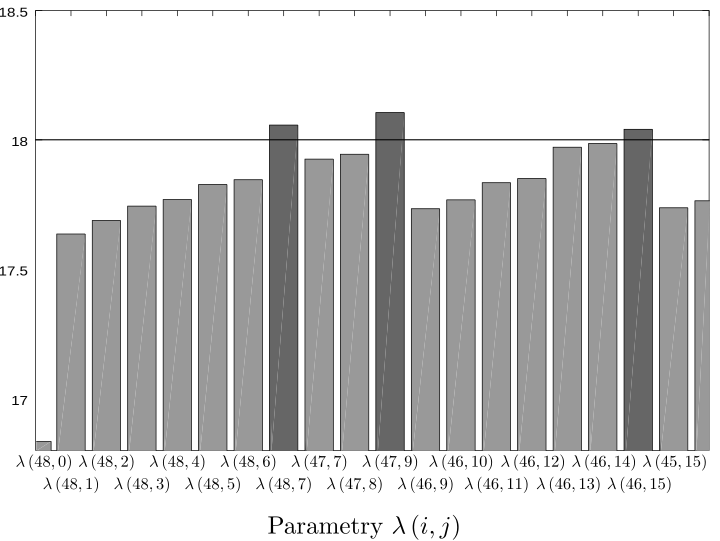
\includegraphics[width=\textwidth]{Chapter_IV/INC_MST_LAMBDA-chart/min}
		\caption{}
		\label{fig:imstdminmax:a}
	\end{subfigure}
	\hfill
	\begin{subfigure}[b]{0.45\textwidth}
		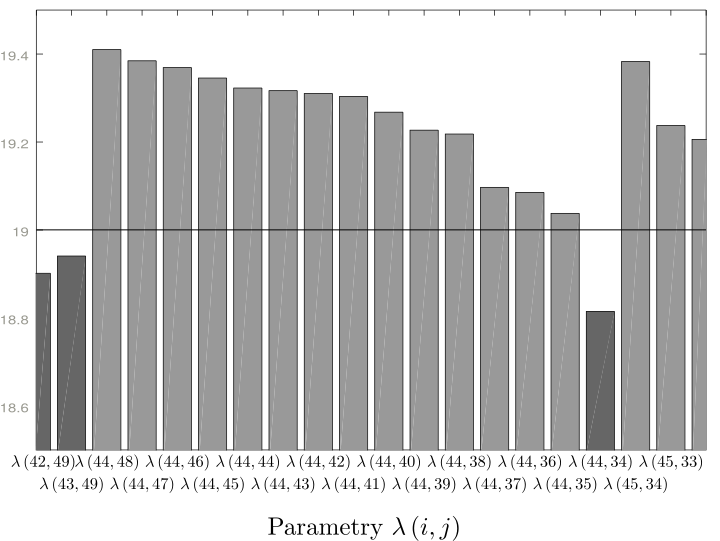
\includegraphics[width=\textwidth]{Chapter_IV/INC_MST_LAMBDA-chart/max}
		\caption{}
		\label{fig:imstdminmax:b}
	\end{subfigure}
	\hfill\null
	\caption{
		Graficzne zaprezentowanie wartości funkcji $d: \NN \times \NN \rightarrow \RR$ dla wycinka algorytmu \ref{alg:imstbinnarysearch2}, obliczającego $\min \left\{ j \; : \; L \leqslant d \left( i, j \right) \right\}$ dla wybranego zakresu wartości indeksów. 
		\textbf{(a)}~Początek proces obliczania kolejnych zmiennych $\text{MinIndex} \left[ i \right]$ dla $i \in \left\{ 48, \dots, 45 \right\}$ ($m^{\prime} = 49$), gdzie jasnym szarym kolorem oznaczono te wartości $d \left( i, j \right)$, dla których nie zachodził warunek $L \leqslant d \left( i, j \right)$. Miejsca oznaczone kolorem ciemniejszym stanowią punkty, w których dla danego $i$ odnaleziono takie $j$, że $j = \min \left\{ j \; : \; L \leqslant d \left( i, j \right) \right\}$ ($L = 18$).
		\textbf{(b)}~Graficzna reprezentacja fragmentu algorytmu obliczającego wyrażenia $\max \left\{ j \; : \; d \left( i, j \right) \leqslant U \right\}$ (od $i = 42$ do $i = 45$). Ciemniejszym kolorem oznaczono wartości funkcji $d \left( i, j \right)$, która dla tak dobranych parametrów, spełnia powyższą nierówność ($U = 19$).
	}
	\label{fig:imstdminmax}
\end{figure}

Opisaną powyższą strategię doskonale ilustruje rysunek \ref{fig:imstdminmax:a}, gdzie wyraźnie widzimy w których momentach wartość indeksu $j$ dla wyrażenia $d \left( i, j \right)$ została na tyle podwyższona, aby przekroczyła wartość dolnego ograniczenia $L$, co pociąga za sobą obniżenie pierwszego parametru i rozpoczęcie procesu od nowa. Analogicznie do schematu wyszukiwania wszystkich wartości $\text{MinIndex} \left[ i \right]$ zachowuje się proces obliczania wyrażeń $\text{MaxIndex} \left[ i \right]$ (przedstawiony na rysunku \ref{fig:imstdminmax:b}) --- opierając o to samo rozumowanie oraz te same własności co powyżej, zaczynając od $i = 1$ oraz $j = m^{\prime}$, możemy tak manipulować obydwoma wartościami, aby całkowity czas operacji nie przekroczył czasu liniowego, zależnego od $m^{\prime}$, podobnie jak miało to miejsce wcześniej. W przypadku rozpoczynania od $j = m^{\prime}$, możemy poczynić niewielką obserwację, że gdy pętla $17$-$21$ w algorytmie \ref{alg:imstbinnarysearch2} zostanie przerwana zanim policzymy $\text{MaxIndex} \left[ i \right]$ dla wszystkich $i \in \left\{ 1\, \dots, m^{\prime} \right\}$, do pozostałych zmiennych możemy przypisać stałą $0$, gdyż taką wartość przyjmie wtedy indeks $j$. Razem z następnymi linijkami, fragment $5$--$26$ stanowi eleganckie usprawnienie bloku $2$-$10$ poprzedniego algorytmu, już znacznie go usprawniając.

Dalsze różnice pomiędzy algorytmami \ref{alg:imstbinnarysearch} a \ref{alg:imstbinnarysearch2} mają charakter bardziej kosmetyczny (usunięcie wywołań rekurencyjnych, zasugerowanie sposobu konstrukcji zbiorów dopuszczalnych par $F$, przerzedzonego zbioru $\mathcal{H}$) i nie wymagają poświęcania im większej uwagi.

\begin{pseudokod}[!htbp]
	\DontPrintSemicolon
	\Begin{
		$\text{MaxIndex} \left[ 0 \right] \leftarrow m^{\prime}$\;
		$\text{MinIndex} \left[ m^{\prime} \right] \leftarrow0$\;
		\While{$L \leqslant U$}{
			$\text{TotalCount} \leftarrow 0$\;
			$i \leftarrow m^{\prime}$\; %zaczynamy od najwiekszego i zjezdzamy w dol (od najwiekszej wartosci d(i,j), dla ktorej j moze byc najmniejsze i L<=)
			$j \leftarrow \text{MinIndex} \left[ i \right]$\; %i spada, więc j'em idziemy w gore, by nie spasc ponizej L. Jesli dojdziemy do jMax, wtedy reszty nie ma co liczyć ,tylko walnąć j - max + 1
			\While{$j \leqslant m^{\prime}$}{
				\While{$L > d \left( i, j \right) \; \wedge \; j \leqslant m^{\prime}$}{
					$j \leftarrow j + 1$\;	
				}
				$\text{MinIndex} \left[ i \right] \leftarrow j$\;
				$i \leftarrow i - 1$\;	
			}
			\For{$i^{\prime} \in \left\{ i, \dots, 1 \right\}$}{
				$\text{MinIndex} \left[ i \right] \leftarrow j$\;	
			}
			
			$i \leftarrow 0$\; %zaczynamy od najmniejszego i idziemy w góre (od najmniejszej wartosci d(i,j), dla ktorej j moze byc najwieksze i <=U)
			$j \leftarrow \text{MaxIndex} \left[ i \right]$\; %i rosnie, więc j'em idziemy w dol, by wejsc powyżej U. Jesli dojdziemy do 0, wtedy reszty nie ma co liczyć ,tylko walnąć j = 0
			\While{$j > 0$}{
				\While{$d \left( i, j \right) > U \; \wedge \; j > 0$}{
					$j \leftarrow j - 1$\;	
				}
				$\text{MaxIndex} \left[ i \right] \leftarrow j$\;
				$i \leftarrow i + 1$\;	
			}
			\For{$i^{\prime} \in \left\{ i, \dots, 1 \right\}$}{
				$\text{MaxIndex} \left[ i \right] \leftarrow 0$\;	
			}
			
			\For{$i \in \left\{ 1, \dots, m^{\prime} \right\}$}{
				\If{$\text{MinIndex} \left[ i \right] \leqslant \text{MaxIndex} \left[ i \right]$}{
					$\text{TotalCount} \leftarrow \text{MaxIndex} \left[ i \right] - \text{MinIndex} \left[ i \right] + 1$\;
				}
			}
			\If{$\text{TotalCount} \leqslant 12 \cdot n$}{
				$F \leftarrow \emptyset$\;
				\For{$i \in \left\{ 1, \dots, m^{\prime} \right\}$}{
					\For{$j \in \left\{ \text{MinIndex} \left[ i \right], \dots,\text{MaxIndex} \left[ i \right] \right\}$}{
						$F \leftarrow F \cup \left( i, j \right)$\;
					}	
				}
				\Return $\textsc{imst-binnary-search} \left( G^{\ast}, T^{\ast}_{\textbf{s}}, \textbf{s}^{\prime}, F, k \right)$\;
			}
			\Else{
				$K \leftarrow \left\lfloor \frac{\text{TotalCount}}{6 \cdot n} \right\rfloor$\;
				$\mathcal{H} \leftarrow \emptyset$\;
				\For{$i \in \left\{ 1, \dots, m^{\prime} \right\}$}{
					$j_{\text{max}} \leftarrow \text{MaxIndex} \left[ i \right]$\;
					\For{$j \leftarrow \text{MinIndex} \left[ i \right]\; ; \;j < j_{\text{max}}\; ; \;j \leftarrow j + K$}{
						$\mathcal{H} \leftarrow \mathcal{H}	\cup \left( i, j \right)$\;
					}
				}
				$\lambda \leftarrow \textsc{median} \left( \mathcal{H} \right)$\;
				$\text{kDiff} \longleftarrow \textsc{get-diff} \left( T \left( \lambda \right), T^{\ast}_{\textbf{s}} \right)$\tcp*{\parbox[t]{3in}{\raggedright Zwróć liczbę krawędzi $e \in T \left( \lambda \right) \setminus T^{\ast}_{\textbf{s}}$.}}
				\uIf{$\text{kDiff} = k$}{
					\Return $T \left( \lambda \right)$\;
				}
				\uElseIf{$\text{kDiff} > k$}{
					$L \leftarrow \lambda$\;
				}
				\Else{
					$U \leftarrow \lambda$\;
				}
			}
		}
	}
	\caption{$\textsc{incremental-mst}^{\prime} \left( G^{\ast}, T^{\ast}_{\textbf{s}}, \textbf{s}^{\prime}, k, L, U \right)$}
	\label{alg:imstbinnarysearch2}
\end{pseudokod}

\section{Analiza poprawności}


fsfdf

d

fdfd

fdf

d

gg

fg

fg

fsfdf

d

fdfd

fdf

d

gg

fg

fg

fsfdf

d

fdfd

fdf

d

gg

fg

fg

\section{Podsumowanie rozdziału}

Wychodząc od funkcji celu, którą otrzymaliśmy w części poświęconej programowaniu liniowemu, w tym rozdziale bardzo dokładnie omówiliśmy proces konstrukcji algorytmu rozwiązującego problem minimalnego drzewa rozpinającego w wersji \textsc{incremental}, pochylając się nad wszystkimi problemami jakie w tym czasie napotkaliśmy i sugerując sposoby ich rozwiązania. Pozwoliło nam to otrzymać bardzo wydajny algorytm, z którego to będziemy korzystać przy próbie przyjrzenia się następnemu problemowi: optymalizacji odpornej z możliwością poprawy rozwiązania, który zdefiniowaliśmy w \ref{eq:rimstdef}. O ile zagadnienie, któremu poświęciliśmy cały ten rozdział, znajduje się jeszcze w zasięgu naszych możliwości obliczeniowych (należy do problemów klasy $P$ --- ma wielomianowy algorytm go rozwiązujący), to któremu będziemy się chcieli przyjrzeć wykracza daleko poza nie~\cite{DBLP:journals/corr/NasrabadiO13}, w związku z czym nasze dalsze rozważania nie skupią się na konstrukcji algorytmu dającego dokładne jego rozwiązania --- będziemy chcieli zaprezentować nieco odmienny punkt widzenia, przedstawiając algorytmy lokalnego przeszukiwania.